\documentclass[a4paper]{report}

\usepackage[english]{babel}
\usepackage[utf8]{inputenc}
\usepackage[sc]{mathpazo}
\usepackage{url}

\usepackage{amsmath}
\usepackage{amsthm}

\usepackage{graphicx}
\usepackage{float}
\graphicspath{{figure/}}
\usepackage{epstopdf}
\usepackage{booktabs}
\usepackage{changes}

\usepackage{hyperref}
\usepackage[numbers]{natbib}   % omit 'round' option if you prefer square brackets
\bibliographystyle{unsrt}
\usepackage{xfrac}

\usepackage{pdfpages}
\usepackage{algorithm}
\usepackage{algorithmic}

\usepackage{amssymb}
\usepackage{color}
\usepackage{booktabs}
\usepackage{multirow}
\usepackage{subfigure}

% \newtheorem{theorem}{Theorem}
% \newtheorem{definition}{Definition}

\newtheorem{myDef}{Definition}
\newtheorem{myTheo}{Theorem}

%%%%%%%%%%%%%%%%%%%%%%%%%%%%%%%%%%%%%%%%%%%%%%%%%%%%%%%%%%%%%%%%%%%%%%%%%

\author{Student name}

\definecolor{sycamoregreen}{RGB}{0,148,68}

\begin{document}
\begin{titlepage}
    \begin{center}
        \vspace*{1cm}

        \huge
        \textbf{Solving Online Mixed-Integer Programming Problems Based on Signal Temporal Logic via a Learning-based Framework}
        \vspace{0.5cm}

        \vspace{1.5cm}
        \Large
        {\color{sycamoregreen}Qi Yi} \\
        \vspace{2cm}
        \large
        Exchange student project \\
        \vspace{2cm}
        Dr.\ Tony A.\ Wood and Prof.\ Maryam Kamgarpour
        \\
        \vspace{5em}
        14/9/2022

        \vfill
        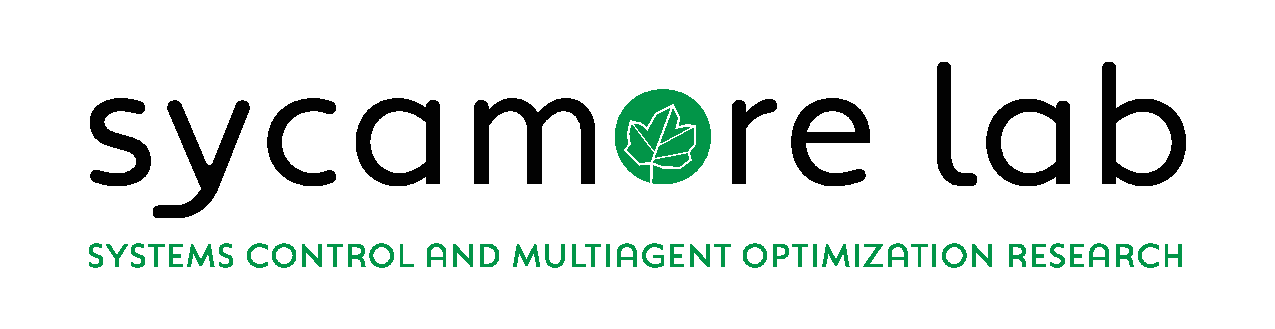
\includegraphics[width=0.9\textwidth]{Sycamore_withtext_DIGITAL_RGB-01.eps}
        \vspace{0.5cm}

        %
        École Polytechnique Fédérale de Lausanne (EPFL)\\
        1015 Lausanne, Switzerland

    \end{center}
\end{titlepage}

\chapter*{Abstract}
To implement complex motion planning tasks, high-level logical behaviors need to be imposed on the robots. Signal temporal logic (STL) provides a convenient way to encode complex motion planning objectives, which can be incorporated into optimization-based motion planning problems formulated as Mixed-Integer Convex Programming (MICP) problems. However, a significant bottleneck encountered is the slow computation for solving such MICPs due to exponential complexity in the number of binary variables. To overcome such difficulties, an efficient STL encoding approach leading to a number of binary variables that is logarithmic in the number of specification predicates is designed via a novel STL tree structure. An Online Mixed-Integer Optimization Based on Signal Temporal Logic (OMISTL) framework, which leverages the cutting-edge machine learning method, is designed to solve the considered problems. By solving numerous MICP instances offline, data is generated and purposefully used to speed up the online solution. Results demonstrate that, compared with the standard STL encoding, the encoding based on the STL tree significantly reduces the number of binary variables used in the problems. And the proposed framework gains speed-ups of 1-2 orders of magnitude in online computation time, which also provides better solutions in terms of feasibility and optimality when compared with the state-of-the-art learning-based methods.


\tableofcontents
% \tableofcontents % create index
%\listoffigures

\chapter{Introduction}
With the advancement of technology and the introduction of increasingly sophisticated autonomous vehicles, such as self-driving cars, delivery drones, and warehouse robots \cite[]{mou2018optimal}\cite[]{sawadsitang2018supplier}\cite[]{liu2022integer}, complex objectives and constraints need to be considered for robotic motion planning problems. Mixed-integer programming (MIP) is a powerful technique to address such problems \cite[]{booth2016mixed}\cite[]{landry2016aggressive}. By modelling discrete control decisions with integer variables, we can, theoretically, solve MIPs to global optimality with branch-and-bound or outer approximation algorithms \cite[]{lee2011mixed}. However, computing the optimal solutions is, in practice, computationally challenging.

When a robot has a more complicated mission than point-to-position navigation from its starting point to the desired destination, it becomes challenging to appropriately formulate the path planning problem. Signal Temporal Logic (STL) specifications define acceptable sequences of the state of the robot, where simple tasks (e.g., reaching or avoiding certain areas) are combined with logic (e.g. visit Area A OR Area B) and temporal conditions (e.g. stay safe in Area C UNTIL going to Area D) to capture complex navigation objectives \cite[]{ulusoy2013optimality}. These specifications can be incorporated into optimization-based motion planning as mixed-integer constraints \cite[]{raman2014model}. 

However, solving MIPs with STL specifications has seen limited application in real-world robotic tasks for the following two reasons:

\begin{itemize}
    \item[$\bullet$] \textit{Inefficient STL encoding}: despite that the standard MIP encoding for STL is sound and complete \cite[]{raman2014model}, it has limited scalability due to exponential computation complexity in the number of binary variables, which may lead to prohibitive computing time to solve the corresponding optimization problems.
\end{itemize}

\begin{itemize}
    \item[$\bullet$] \textit{Slow computation times}: it is still challenging to solve MIPs in online settings where real-time computations are crucial. For example, a model predictive control (MPC) problem requires sampling the states of robots and returning the solution within a few milliseconds \cite{ding2022trajectory}, while typical solution times range from seconds to minutes.
\end{itemize}

This is why there is still a large gap between STL motion planning modeling and the real-world implementation of MICP-based controllers. To fill this gap, in this project, we leverage the idea that by solving numerous MICP instances, one can generate a large amount of offline data that can be purposefully used to accelerate online solutions significantly. By developing an efficient STL encoding, this learning-based approach can be combined with STL specifications and deal with more general cases in robotics systems. 


\section{Contributions}

This project proposes an Online Mixed-Integer Optimization Framework Based on Signal Temporal Logic (OMISTL), which can be used to solve mixed-integer programming problems formulated by STL in such scenarios that the solutions must be returned in real-time reliably and at a very high speed. For instance, MPC control for robot motion planning requires the algorithm to solve mixed-integer convex problems between each sampling time (maybe less than 0.1s), which cannot be realized with state-of-the-art solvers such as the Gurobi. An efficient STL encoding approach leading to a number of binary variables that is logarithmic in the number of specification predicates is designed via a novel STL tree structure.

Another application is to speed up the computation for solving the general STL planning problems considering robustness satisfaction, which may require prohibitive computing time because it contains many mixed-integer constraints to satisfy complex navigation objectives.

In this project, we present the contributions from two perspectives:

Compared with previous STL encoding approaches:

\begin{itemize}
    \item[$\bullet$]An model-predictive controller and an STL planner based on the proposed OMISTL are developed. 
    \end{itemize}

    \begin{itemize}
        \item[$\bullet$]An efficient STL encoding approach leading to a number of binary variables that is logarithmic in the number of specification predicates is designed via a novel STL tree structure, where a formula flattening method is applied to simplify the tree.
        \end{itemize}

    \begin{itemize}
        \item[$\bullet$]While the previous STL tree only decomposes the specification as $\wedge$-type nodes and $\vee$-type nodes, the proposed method can further decompose these nodes with repeated structure.
            \end{itemize}
    \begin{itemize} 
        \item[$\bullet$]Numerical examples show that the OMISTL framework demonstrates speed-ups of 1-2 orders of magnitude when solving MICP online compared with the state-of-the-art STL encoding, which
        can realize real-time control efficiently and reliably.
    \end{itemize}

Compared with previous approaches based on machine learning:

\begin{itemize} 
    \item[$\bullet$]Compared with work \cite{bertsimas2022online}, the static LQR model is extended into a real-time MPC model combined with STL specification, which is computing online in a receding horizon with time-varying destinations and initial conditions.
\end{itemize}

\begin{itemize} 
    \item[$\bullet$]With the proposed efficient STL encoding, we define a more succinct and general STL integer strategy used for the classification compared with \cite{bertsimas2022online}\cite{Cauligi2020}, which enables OMISTL framework to be combined with different STL specifications. In addition, the fewer tight constraints and integer strategies are obtained through our definition, which contribute to the online computation.
\end{itemize}

\begin{itemize}
    \item[$\bullet$]The number of binary variables is reduced from typical $TN_f$ to $T\log_2(N_f)$ for obstacle avoidance application, where T is the STL time horizon, $N_f$ is the number of the obstacle faces. And from $TN^\pi$ to $\sum_{1}^{N^\lor}(\log_2(N_i+1))$ for general STL, where $N_i$ is the number of subformulas for the $i_{th}$ disjunctions, and $N_{\pi}$ is the number of predicates.
\end{itemize}

\begin{itemize} 
    \item[$\bullet$] The results show that the OMISTL framework reports more than 90\% feasible solutions and better solutions (92\% optimal), compared with the existing learning-based methods. The online acceleration mainly depends on the integer variables and disjunctions of STL formulas.
\end{itemize}

\section{Related work}
\subsection{Motion planning by MIP}
One of the classical works treating the motion planning problems is in \cite[]{earl2005iterative}, which introduces an iterative MILP algorithm that addresses the issues of MILP coping with large-scale models. Therein, two problems are considered: trajectory-generation with obstacle-avoidance requirements and minimum-time trajectory-generation problems. The motion planning topic is also investigated in \cite{cetin2007hybrid}, where the addressed problem is the generation of collision-free trajectories for the reconfiguration of spacecraft formations. The “big-M” technique is used to write the parametrized optimization as a MILP whose solution can be obtained using standard MILP solvers. In \cite[]{richards2003performance}, MILP has been used for open-loop vehicle trajectory design, enabling the inclusion of non-convex constraints such as plume impingement avoidance.

It is generally accepted that the collision avoidance problem is a challenging task due to the presence of the non-convex feasible domain. The work of \cite[]{culligan2006online} presents a path planner using MIP to solve a receding horizon optimization problem for unmanned aerial vehicles (UAVs), where the obstacle avoidance constraints for the MILP formulation are considered. In \cite[]{schouwenaars2006safe} the author presents a framework for safe online trajectory planning of unmanned vehicles through partially unknown environments. An MPC framework is employed, MIP playing an instrumental role in order to incorporate the collision avoidance constraints. These problems can be extended into multiple obstacles cases, which can be found in \cite[]{maia2009use}\cite[]{stoican2018exact} \cite[]{richards2015inter}.
However, the above studies fail to extend the considered problems into more general STL problems since obstacle avoidance and reaching area is just the essential tasks in robotics control and the simple cases in STL specifications. To implement more complex tasks, STL must be combined with the MIP problems to make the robots intelligent.
\subsection{STL specification encoding} 
The standard STL encoding uses Mixed-Integer Convex Programming (MICP) is first proposed in \cite[]{raman2014model}. And later refined in \cite[]{sadraddini2015robust} and \cite[]{sadraddini2018formal}, which is sound and complete, and enable us to find globally optimal solutions. However, the major limitation is and slow computation and scalability. MICP’s worst-case complexity is exponential in the number of binary variables, and the standard STL synthesis introduces a binary variable for each predicate at each timestep, which limits MICP methods to simple specifications and short time horizons. With
this in mind, much research in STL synthesis has gone toward reducing MICP problem sizes. For example, rewriting formulas in Positive Normal Form (PNF) significantly reduces the number of binary variables and constraints \cite[]{raman2014model}, \cite[]{sadraddini2018formal}. Waypoint-based abstractions can further limit the problem
size \cite[]{conforti2014integer}.

Another possibility is to formulate MICPs with tighter convex relaxations. While this does not improve the worst-case complexity, a tighter convex relaxation increases branch-and-bound efficiency and often improves performance in practice \cite[]{conforti2014integer}. This approach has been pursued for Metric Temporal Logic in \cite[]{kurtz2021more} and piecewise-affine reachability in \cite[]{marcucci2021shortest}. Much STL research in recent years has focused on avoiding MICP entirely and instead designing efficient heuristic methods
which are sound but not complete. Such methods include gradient-based optimization \cite[]{gilpin2020smooth} \cite[]{mehdipour2019arithmetic} \cite[]{leung2020back}, differential dynamic programming \cite[]{kurtz2020trajectory} and control barrier functions \cite[]{lindemann2018control}. These approaches improve scalability, especially concerning the specification time horizon, but offer limited formal guarantees and often struggle to handle more complex specifications. What's worse, the most tricky issue remains, i.e. solving the MICPs combined with STL online, which satisfies the requirement of real-time control in practice.
\subsection{Learning-based approach for online optimization}
Recently, there has been a surge of interest in applying learning-based methods to accelerate solution times for optimization-based controllers. In \cite[]{chen2022large}\cite[]{zhang2019safe}, neural networks are used to warm start a solver for a QP-based controller used in a receding horizon fashion. Tang, et al.\cite[]{tang2018learning} also consider nonconvex optimization-based controllers by learning warm starts for an SQP-based trajectory optimization library and for indirect optimal control methods \cite[]{tang2019data}. Using tools from differentiable convex optimization, a learning-based approach to tune optimization-based controllers is proposed in \cite[]{agrawal2020learning}. While these methods have shown considerable promise, they only consider the setting of continuous optimization.

Relatively less attention has been paid to using data-driven
techniques for accelerating integer program solutions in control \cite[]{bengio2021machine}\cite[]{lodi2017learning}. A popular class of methods has been to pose branch-and-bound as a sequential decision-making process and apply imitation learning to learn effective variable and node selection strategies \cite[]{khalil2017learning}\cite[]{he2014learning}. However, these approaches can still be too computationally expensive for applications in control, as they require solving branch-and-bound and computing multiple forward passes of a neural network online.

Masti and Bemporad \cite[]{masti2019learning} use a regression-based approach to train a neural network to learn binary variable assignments. However, the authors only demonstrate this approach on a MIQP with 14 binary variables. An approximate dynamic programming approach is presented in \cite[]{deits2019lvis}, where the cost function for a MIQP controller is learned. However, the approach still requires solving an expensive MIQP using branch-and-bound online. To the best of the author's knowledge, there is no existing learning-based method that tries to extend the motion planning problems into STL cases.

\section{Notation}

$x$: continuous decision variables\\
$\delta$: binary variable\\  $\delta^\pi$: binary variable used for the predicate\\ 
$\delta^{\pi*}$: the optimal solution of $\delta^\pi$ \\ 
$\delta^*$: the optimal solution of the binary variable\\
$\theta^\varphi$: problem parameter depending on the STL specification $\varphi$\\
$f_0$: objective function\\
$f$: linear constraints that only contain the continuous variables\\
$g$: mixed-integer constraints that contain binary variables\\
$g^\pi$: big-M constraints used for the predicate $\pi$\\
$\pi$: predicates\\
$\varphi$: STL specification\\
$m_c$: number of linear continuous constraints \\
$m_I$: number of mixed-integer constraints,
$\mathcal{S}(\theta)$: integer strategy\\
$\mathcal{T}(\theta)$: the set of active inequality constraints,
$\mathcal{S}(\theta^\varphi)$: STL integer strategy \\
$\mathcal{S}_i(\theta^\varphi)$: $i_{th}$ STL integer substrategy \\
$s_j$: $j_{th}$ label,
$\mathcal{T}^\pi$: the set of tight constraints\\
$X_{SOS1}$: SOS1 encoding from the values of binary variables\\
$y$: signal sequence\\
$\rho^\varphi$: STL robustness measure,
$T$: time horizon\\
$N_i$: number of subformulas for the $i_{th}$ disjunction \\
$N^\pi$: number of predicates\\
$N^\vee$: number of disjunctive subformulas\\
$E^\varphi$: an STL tree consists of a tuple$(C, \tau, o, \rho^\varphi)$, where  $C = [E^\varphi_1,E^\varphi_2,...,E^\varphi_N]  $ is a list of $N$ subtrees, $\tau $ is a list of time steps corresponding to the $N$ subformulas, $o \in \{ \wedge, \vee\}$ is the combination type\\
$x_t$: system state at timestep t\\ 
$u_t$: control input at time t\\
$y_t$ is the output signal at time t\\
$X$, $U$, $Y$: convex sets\\
$A, B, C, D$: matrices of appropriate dimension\\
$x_0$: initial position\\
$v_0$: initial velocity\\
$x_g$: desired state\\
$v_g$: desired velocity\\
$Q\succeq 0,R\succeq 0 $: symmetric cost matrices\\
$n$: number of the obstacles\\
$N$: number of subformulas\\
$N_f$: number of faces of a single obstacle\\
$T$: STL formula horizon\\
$O_i$: $i_{th}$ obstacle\\
$X_i^o$: coordinates of each obstacle \\
$X^{oh}$: a one-hot code. \\
$\mathcal{S}_{i,j}(\theta^{\varphi})$: substrategy of $\mathcal{S}_{i}(\theta^{\varphi})$ after decomposition\\
$\mathcal{T}^{\pi}(\theta_{i,j}^{\varphi})$: the index of tight constraints\\
$X_{i,j}^{SOS1}$: the SOS1 encoding with the corresponding obstacle $i$ for sample $j$\\

\section{Technical background}


\subsection{Signal Temporal Logic}

It is clear that any temporal logic formula can be brought into the negation normal form \cite[]{baier2008principles}, where
all negation connectives appear immediately before a predicate. And we can further remove the negations of predicates by simply reversing the inequalities to make it in Positive Normal Form (PNF), which reduces the number of binary variables and constraints \cite{2019Formal}.
We consider STL formulas over convex predicates in PNF, the syntax of STL is defined as : 

\begin{equation}
\varphi:=\pi|\bigvee_{i} \varphi_{i}| \bigwedge_{i} \varphi_{i}|\square_{\left[t_{1}, t_{2}\right]} \varphi| \diamond_{\left[t_{1}, t_{2}\right]} \varphi \mid \varphi_{1} \mathcal{U}_{\left[t_{1}, t_{2}\right]} \varphi_{2},
\end{equation}
where predicates $\pi$ are defined by convex functions: $ g^\pi: Y \rightarrow \mathbb{R}$ such that $\{y|g^\pi(y)\leq 0\} $ are convex sets. In this report we consider only bounded-time specifications, i.e., those with $t_2$ finite. Note that such convex predicates include linear ones $g^\pi (y_t) = a^Ty-b$.

The STL formulas are defined recursively as follows, where we denote the fact that signal $y$ satisfies specification $\varphi$ as $y \models \varphi $:
\begin{equation}
    \begin{array}{lll}(y, t) \models \mu & \Leftrightarrow & \mu(y(t))>0 \\ (y, t) \models \varphi \wedge \psi & \Leftrightarrow & (y, t) \models \varphi \wedge(y, t) \models \psi \\ (y, t) \models \varphi \vee \psi & \Leftrightarrow & (y, t) \models \varphi \vee(y, t) \models \psi \\ (y, t) \models \square_{[a, b]} \varphi & \Leftrightarrow & \forall t^{\prime} \in[t+a, t+b],\left(y, t^{\prime}\right) \models \varphi \\ (y, t) \models \varphi \mathcal{U}_{[a, b]} \psi & \Leftrightarrow & \exists t^{\prime} \in[t+a, t+b] \text { s.t. }\left(y, t^{\prime}\right) \models \psi \\ & & \wedge \forall t^{\prime \prime} \in\left[t, t^{\prime}\right],\left (y, t^{\prime \prime} \right) \models \varphi\end{array}
\end{equation}

To measure how strongly a formula is satisfied by a signal,
here we present the quantitative semantics of STL, which defines a scalar “robustness value” $\rho^ \varphi(y)$ which is positive only if $y \vDash \varphi$. 
Positive robustness indicates satisfaction, and negative robustness indicates violation:

\begin{equation}
    \label{robustness definition}
    \begin{array}{lll}
    \boldsymbol{y} \vDash \varphi & \Leftrightarrow & \rho^{\varphi}((\boldsymbol{y}, 0)) \geq 0 \\

    \rho^{\pi}((\boldsymbol{y}, t)) & = & -g^{\pi}\left(\boldsymbol{y}_{t}\right) \text {, since } \boldsymbol{y} \vDash \pi \text { if } g^{\pi}\left(\boldsymbol{y}_{0}\right) \leq 0 \\

    \rho^{\varphi_{1} \wedge \varphi_{2}}((\boldsymbol{y}, t)) & = & \min \left(\rho^{\varphi_{1}}((\boldsymbol{y}, t)), \rho^{\varphi_{2}}((\boldsymbol{y}, t))\right) \\

    \rho^{\varphi_{1} \vee \varphi_{2}}((\boldsymbol{y}, t)) & = & \max \left(\rho^{\varphi_{1}}((\boldsymbol{y}, t)), \rho^{\varphi_{2}}((\boldsymbol{y}, t))\right) \\

    \rho^{\Diamond_{\left[t_{1}, t_{2}\right]} \varphi^{\prime}}((\boldsymbol{y}, t)) & = & \max _{t^{\prime} \in\left[t+t_{1}, t+t_{2}\right]}\left(\rho^{\varphi}\left(\left(\boldsymbol{y}, t^{\prime}\right)\right)\right)\\

    \rho^{\square_{\left[t_{1}, t_{2}\right]} \varphi^{\prime}}((\boldsymbol{y}, t)) & = & \min _{t^{\prime} \in\left[t+t_{1}, t+t_{2}\right]}] \left(\rho^{\varphi} \left( \left( \boldsymbol{y}, t^{\prime} \right) \right) \right)\\

    \rho^{\varphi_{1} \mathcal{U}_{\left[t_{1}, t_{2}\right]} \varphi_{2}}((\boldsymbol{y}, t)) & = & \max _{t^{\prime} \in\left[t+t_{1}, t+t_{2}\right]}\left(\operatorname {min} \left(\left[\rho^{\varphi_{1}}\left(\left(\boldsymbol{y}, t^{\prime}\right)\right), \right.\right.\right. \\ 
    & &
     \min _{ t^{\prime \prime} \in [t+t_{1}, t^{\prime}]} 
     \left.\left.\left.\left(\rho^{\varphi_{2}}\left( \left( \boldsymbol{y}, t^{\prime \prime}\right)\right)\right) \right] \right) \right)

    \end{array}
    \end{equation}

For a given STL formula , we denote the time horizon as $T$, the number of predicates as $N^\pi$ and the number of disjunctive subformulas as $N^\vee$, here we introduce the definition of disjunctive (sub)formulas:

% \begin{equation}
%     \begin{array}{lll}
%         \pi, \bigwedge_{j=1}^{n} \varphi_{i} \text{, and } \square _{\left[t_{1}, t_{2}\right]} \varphi_{i} \text{ are not disjunctive;}\\
%         \bigvee_{j=1}^{k} \varphi_{i} \text{is disjunctive, with $k$ disjunctions;}\\
%         \Diamond_{\left[t_{1}, t_{2}\right]} \varphi \text{ is disjunctive, with } t_{2}-t_{1} \text{disjunctions;}\\
%         \varphi_{1} \mathcal{U}_{\left[t_{1}, t_{2}\right]} \varphi_{2} \text{ is disjunctive, with } t_{2}-t_{1} \text{ disjunctions }
%     \end{array}
% \end{equation}

\begin{myDef}
    Disjunctive (sub)formulas are defined as follows:\\
    1) $\pi, \bigwedge_{j=1}^{n} \varphi_{i}$, and $\square_{\left[t_{1}, t_{2}\right]} \varphi_{i}$ are not disjunctive;\\
    2) $\bigvee_{j=1}^{k} \varphi_{i}$ is disjunctive, with $k$ disjunctions;
    $\Diamond_{\left[t_{1}, t_{2}\right]} \varphi$ is disjunctive, with $t_{2}-t_{1}$ disjunctions;\\
    3) $\varphi_{1} \mathcal{U}_{\left[t_{1}, t_{2}\right]} \varphi_{2}$ is disjunctive, with $t_{2}-t_{1}$ disjunctions.
\end{myDef}


We denote the number of disjunctions associated with the $i_{th}$ disjunctive subformula as $N_i$. For instance, the formula $ (a\vee b)\wedge \Diamond_{[0,T]}c$ has two disjunctive subformulas, with $N_1=2$ and $N_2=T+1$ respectively.

\subsection{Mixed-integer programming}

In this work, the  STL motion planning problem is formulated as the parameterized mixed-integer convex programs (MICP). Given the STL specification $\varphi$, the general form is:

\begin{equation}
    \label{eq1}%问题编号
    \begin{aligned}
        \min \quad       & f_0(x,\delta;\theta^\varphi )        \\
        \text{s.t.}\quad &
        f_i(x;\theta^\varphi ) \leq 0, \quad i=1,...,m_c,        \\                                         &
        g_i(x,\delta_i ;\theta^\varphi ) \leq 0, \quad i=1,...,m_I
        \\
                         & \delta \in(0,1)^{n_{\delta}},
    \end{aligned}
\end{equation}
where $x \in \mathbb{R} ^{n_{x}}$ are continuous decision variables, $\delta \in(0,1)^{n_{\delta}} $ are binary variables, and $\theta^\varphi \in \mathbb{R} ^{n_{p}}$ are the problem parameters depending on the STL specification $\varphi$. The linear constraints $f_i$ only contain the continuous variables $x$, and $g_i$ are all the mixed-integer constraints that contain binary variables $\delta_i$. 

Formulating STL specification using mixed-integer constraints $g_i$ poses a challenge for this problem, where $g_i$ includes the Big-M constraints and SOS1 constraints. Via the STL tree structure in \cite{kurtz2022mixed}\cite{leung2020back}, Big-M constraints and SOS1 constraints enable us to create mixed-integer constraints to capture all STL specifications with a logarithmic number of binary variables, which is clarified in section \ref*{STL_planner}. Big-M constraints are used for the predicates $\pi$ of the STL specification $\varphi$, and SOS1 constraints are introduced for the nodes of the STL tree. For the specific encoding method please refer to section \ref*{STL_encooding}.


\subsubsection*{Big-M constraint}
Big-M constraints are a regular source of instability for optimization problems. In this paper Big-M method is used to formulate the disjunctive predicates. Let $N_\vee^{\pi}$ be the number of disjunctive subformulars for predicates (indexed by $i$), and $N_i$ be the number of disjunctions associated with the $i_{th}$ disjunctive subformula (indexed by $j$). The $j_{th}$ predicates for the $i_{th}$ disjunctive subformulars can be expressed as:

\begin{equation}
    \bigvee_{j=1}^{N_i} a_{ij}^Tx+b_{ij}>0,
\label{linear_predicates}
\end{equation}
where $a_{ij} \in \mathbb{R} ^{n_{x}} $ and $b_{ij} \in \mathbb{R}$ difine the $i_{th}$ disjunctive subformulars $j_{th} $ predicates.
To make the forms consistent we denote a linear predicate $\pi$ by convex functions $g^\pi
:\mathbb{R}^{n_x} \rightarrow \mathbb{R}$, i.e. $a_{ij}^Tx+b_{ij}>0 \Leftrightarrow  g_{ij}^\pi(x;\theta^\varphi)<0$ where $a_{ij}$ and $b_{ij}$ are included into the problem parameters $\theta^\varphi$ depending on $\varphi$.
 

% rewrite the big-M formulation according to Vasileio's paper

It is known that satisfaction of a series of disjunctive predicates as in \ref*{linear_predicates} as can be equivalently written as \cite{Maryam2019}:

\begin{equation}
\bigvee_{j=1}^{N_i} a_{ij}^Tx+b_{ij}>0 \Leftrightarrow \bigwedge_{j=1}^{N_i}a_{ij}^Tx+b_{ij}+M(1-\delta_{ij})>0,
\end{equation}
where $\delta_{ij} \in \{0,1\}$ is a binary variable, which implies $a_{ij}^Tx+b_{ij}>0$ when $\delta_{ij}=1$, and renders the constraint trivial when $\delta_{ij}=0$. $M$ is a large coefficient that is chosen to be larger than any reasonable value that a continuous variable or expression may take. 
Since it must hold that at least one of the $\delta_{ij}$ is equal to 1 for the $i_{th}$ subformulars, a constraint $\sum_{j=1}^{N_i} \delta_{ij} \geq 1$ is added as well. 

For an example, use Big-M constraint to formulate a obstacle avoiding STL formula $\varphi := \lnot O $ for robots in a 2-D position $(p_1,p_2)$. Then four disjunctive predicates are needed as shown in fig.\ref*{big_M}:

%Q: check this. if delta1 = 0, then p1-a >= M. is this what you want?
%Re: Yes, this expression is actually the same as Vasileio's paper, depending on you how choose \delta=1 or 0 to make the constraint hold or not. Here we use  delta=0 to imply p1-a+M>=0 so that it doesn't hold. 

\begin{equation}
    (p_1 \geq a) \vee (p_1 \leq c) \vee (p_2 \geq b) \vee (p_2 \leq d),
\end{equation}
thus 4 binary variables $\delta_1 - \delta_4 $ are introduced with Big-M constraints: 
\begin{equation}
\begin{split}
    \mathrm{p}_1-a + M^+\left(1-\delta_1\right)\geq 0,
    \quad \mathrm{p}_1-c + M^-\left(1-\delta_3\right) \leq 0, \\
    \mathrm{p}_2-b + M^+\left(1-\delta_2\right) \geq 0, \quad \mathrm{p}_2-d + M^-\left(1-\delta_4\right) \leq 0,
\end{split}
\end{equation}
where $M^+,M^-$ are sufficient large positive/negetive numbers. $\delta_1 = 1$ implies $p_1 \geq a$ so that the linear predicate holds and force the robot to go above the face $a$, while $\delta_3 = 0$ implies $p_1 - c +M^-\leq 0$, rendering itself a trivial constraint. To avoid a 4-face obstacle, we need at least one predicate to be held, so adding the constraint $\delta_1+\delta_2+\delta_3+\delta_4 \geq 1$.


\begin{figure}
    \vspace{0.5cm}
    \centering
    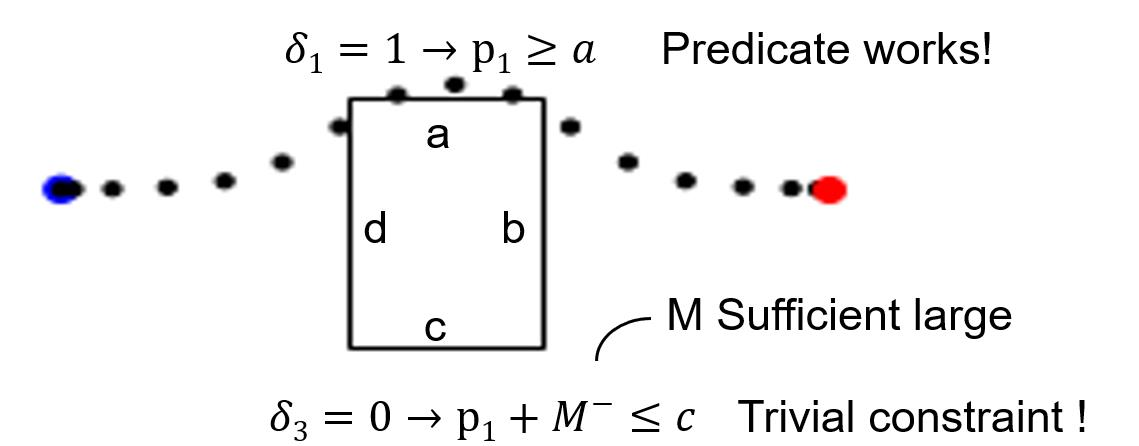
\includegraphics[scale=0.4]{big_m.jpg}
    \vspace{-0.4cm}
    \caption{Introducing binary variables for Big-M constraints}
    \label{big_M}
    \vspace{-0.6cm}
\end{figure}

\subsubsection*{Tight constraint}
The definitions of tight constraints vary from problem to problem, where the names may also change (active/tight/binding constraints).    Finding the set of tight constraints contributes to accelerating solving the problem because one can ignore the other redundant constraints.  How to define the tight constraints determines choosing which redundant constraints to be neglected.
\subsubsection*{A. Previous definition of tight constraints}
According to the most common and basic definition in \cite[]{bertsimas2022online}, tight constraints are a set of active inequality constraints, which are defined as:
\begin{equation}
\label{tight1}
    \mathcal{T}(\theta)= \{i|f_i(x^*,\theta)=0,g_i(x^*,\delta^*,\theta)=0\},
\end{equation}
here tight constraints mark these constraints that are equalities at optimality, so that others are redundant for the original problem, removing them does not change the optimal solutions. 

% For the non-degenerate problems, the tight constraints are corresponding to the support constraints. Removing the support constraints would allow a decrease in object functions \cite{calafiore2010random}(definition 2.1), while removing the non-tight constraints, the optimal solution would not change.

% With degenerate problems, we can have more tight constraints than support constraints for an optimal solution $x^*$. This is because the support constraints set is no longer unique in case of degeneracy.
% However, the set of tight constraints in \ref{tight1} remains unique, because this tight constraint definition is independent from support constraints, it refers to all the constraints that are satisfied as equalities. 

Another definition of tight constraints \cite[]{Cauligi2020} can be used to deal with more general class of MICP in robotics, which are defined as:

\begin{equation}
\label{tight2}%问题编号
    \begin{aligned}
        \mathcal{T}_M(\theta)=\left\{i \mid g_i\left(x^* ; \theta\right) \leq a_i(\theta) \delta_i \Longleftrightarrow \delta_i=\delta_i^*\right\},
    \end{aligned} 
\end{equation}
where $g_i(x^* ; \theta) \leq a_i(\theta) \delta_i$ is the genenral form of Big-M constraint, and this means for the particular continuous solution $x^*$, this constraint can only be satisfied by the values from the optimal integer solution $\delta^*$. This definition avoids the there existence of multiple optimal strategies, and there is no association with the previous definition \ref*{tight1}.

% For instance, suppose we have $g(x^*,\theta)\leq 0$ for some particular continuous solution $x^*$, so that the inequality can be satisfied by both $\delta^{*}=0$ and  $\delta^{*}=1$, making $\delta^{*}$ not unique therefore it is not tight. 
\subsubsection*{B. Our definition of tight constraints}
In this work, based on the properties of Big-M constraints and STL tree, we propose a definition of tight constraint $\mathcal{T}^\pi$ for the predicate of each leaf in the STL tree:

\begin{myDef} Tight constraints.
\label{tight3}%问题编号
    For the particular continuous solution $x^*$, the tight constraints $\mathcal{T}^\pi$ refer to the convex functions $g^\pi$ 
    of predicate $\pi$, which can be satisfied by the values from the integer solution $\delta^{\pi*}$, which is formulated by:
    \begin{equation}
        \begin{aligned}
            \mathcal{T}^\pi(\theta^\varphi) = \{i|g_i^\pi(x^*;\theta^\varphi) \leq M(1-\delta_i^{\pi*}) 
            \Longrightarrow 
            g_i^\pi(x^*;\theta^\varphi) \leq 0\}
        \end{aligned}
    \end{equation}
\end{myDef}

To avoid confusion, from now on all the tight constraints in the following text are referring to definition \ref*{tight3}, which means for an optimal solution $x^*$ and $\delta^{\pi*}$, the tight constraints imply that the linear constraints of the predicates $g_i^{\pi}$ are less equal than 0.

The insight behind the definition is easy: based on the big-M method, $\delta^{\pi*}=0$ implies trivial constraints that can be neglected when solving MIPs. And tight constraints choose these non-redundant constraints that may form the boundary of the optimal solutions, corresponding to $\delta^{\pi*}=1$. Note that the tight constraint is defined based on the predicate $\pi$ only because the big-M constraints are merely used in the leaf nodes.

By introducing the set of tight constraints, the goal is to define a unique strategy set for each parameter sampling, and use it as labels in the machine learning. Since given a sampling parameter $\theta$, the MICP problem may have multiple optimal integer solutions, leading to multiple correct labels so that the classification problem becomes ill-posed.
%Q:explain why for the machine learning training you need a unique set

Definition \ref{tight3} guarantees a unique strategy from a solution $(x^*,\delta^*)$ as well, because we consider only one of the optimal solutions to be $\delta^*$ since it is enough for training purposes. Note that most solvers such as Gurobi return anyway only one solution and not the complete set of optimal solutions. And with one solution $(x^*,\delta^*)$, we can always define a unique strategy using the definition \ref{tight3}.

Compared with \ref*{tight1} and \ref*{tight2}, definition \ref{tight3} is easier to be obtained even without computation, just record the values from the binary variables. Although definition \ref*{tight3} has no relationship with definition \ref*{tight2}, it includes the scenarios in defintion \ref*{tight1}. Because definition \ref*{tight1} can be satisfied when $\delta = 1$ and we can further label these constraints that hold equalities at optimality, and it cannot be satisfied with $\delta = 0$ since the equality cannot be realized with the big M value.

%%say it before introducing the tight constraint, use subpara to seperate
 
\subsubsection*{STL integer strategy}  

According to the idea of the optimal strategy in \cite{bertsimas2022online},  the integer strategy $\mathcal{S}(\theta)$ is a tuple $(\delta^*(\theta),\mathcal{T}(\theta))$, where $\delta^*$ is the optimal binary solution of the problem (\ref*{eq1}), and $\mathcal{T}(\theta)$ is the corresponding set of tight constraints.

A program is defined to be well-posed if it admits a unique continuous minimizer $x^*$ \cite{Cauligi2020}\cite{jaynes1973well}, but has possibly multiple discrete optimizers ${\delta^*}$. The problem considered is assumed to be well-posed because MICP is non-convex and admits multiple global optima. Naively using the integer strategies from \cite{bertsimas2022online}\cite{bertsimas2021voice} may lead to a pitfall that for the same sampling data $\theta^\varphi$, we may have an ill-posed supervised learning problem with multiple correct labels. The definition \ref{tight3} avoids the existence of multiple optimal strategies ${(\delta^{\pi*},\mathcal{T}^\pi(\theta^\varphi))}$ for a well-posed problem, because by fixing $\delta^\pi$ to its optimal value $\delta^{\pi*}$, there is only one unique tight constraint.

The number of binary variables $\delta^\pi$ may increase exponentially with the STL specification $\varphi$, simply taking them as the components of the integer strategies in \cite{Cauligi2020} will result in a complex classification task. To ameliorate this issue, first we leverage the STL tree structure to decompose the strategies, and then SOS1 encoding is developed to represent the optimal solution with fewer binary variables. At last, the STL integer strategy is defined as:
\begin{myDef}
    STL integer strategy. STL integer strategy $\mathcal{S}(\theta^\varphi)$ is a tuple which contains the index of tight constraints $\mathcal{T}^\pi(\theta^\varphi)$ of an STL motion planning problem, and the values of the integer variables which is encoded as SOS1 encoding $X^{SOS1}$:
    \begin{equation}
        \label{integer strategy}
        \begin{aligned}
            \mathcal{S}(\theta^\varphi) =(\mathcal{T}^\pi(\theta^\varphi), X^{SOS1}), 
        \end{aligned}
    \end{equation}
\end{myDef}
$\mathcal{T}^\pi(\theta^\varphi)$ is the index of the tight constraint, and $X^{SOS1}$ is the SOS1 encoding of the integer variable values of $\delta$ with fewer logarithmic binary variables, which is clarified in section \ref{Decomposition for MPC}. Note that compared with \cite{bertsimas2022online}\cite{Cauligi2020}\cite{bertsimas2021voice}, this integer strategy is a less complex and more general form that can be extended into STL scenarios, because the problem they considered is just a special case that simply takes conjunction of several predicate formulas.

With the given integer strategy $\mathcal{S}(\theta^\varphi)$, the SOS1 encoding $X^{SOS1}$ can be decoded and recover the optimal solution of integer variables $\delta^*$, the set of tight constraints is determined as well, so that the MICP problem (\ref*{eq1}) can be simplified as such form:
\begin{equation}
    \label{reduced_problem}%问题编号
    \begin{aligned}
        \min \quad       & f_0(x;\delta^*,\theta^\varphi )        \\
        \text{s.t.}\quad &
        f_i(x;\theta^\varphi) \leq 0, \quad i=1,...,m_c     \\                                         &
        \hat{g_i}(x,\delta_i;\theta^\varphi) \leq 0, \quad i \in \mathcal{T}^\pi(\theta^\varphi)
        \\
                         & \delta = \delta^*(\theta^\varphi),
    \end{aligned}
\end{equation}
compared with the original MICP (\ref{eq1}), solving problem (\ref{reduced_problem}) is much easier because it is continuous, convex and has fewer constraints. In fact, if the original problem is a MIQP/MICP, solving (\ref{reduced_problem}) is equal to solving a set of linear equations defined by the KKT conditions.


\chapter{Problem Formulation}
\section{System Definitions}
In this report, We consider discrete-time linear dynamics:
\begin{equation}
    \begin{aligned}
    \label{system dynamics}
    x_{t+1} = Ax_t+Bu_t,\\
    y_t = Cx_t + Du_t,
    \end{aligned}
\end{equation}
where $x_t \in X \subseteq  \mathbb{R}^{n_x}$ is the system state at timestep $t \in \mathbb{N}$, $u_t \in U \subseteq  \mathbb{R}^{n_u}$ is the control input, and $y_t \in Y \subseteq \mathbb{R}^{(n_x+n_u)}$ is the output signal. $A \in \mathbb{R}^{n_x \times n_x}$, $B \in \mathbb{R}^{n_x \times n_u}$ are the system dynamics' matrices, $C \in \mathbb{R}^{(n_x+n_u) \times n_x}$, $D \in \mathbb{R}^{(n_x+n_u) \times n_u}$ are matrices to generate the output signals $y_t = [x_t,u_t]$.We assume that the states, the inputs and outputs are constrained to convex sets $X$, $U$ and $Y$. 

Given a finite horizon length $T$, an initial state $x_0$ and a control sequence $u = (u_0, u_1,...,u_{T-1})$, the evolution of the state trajectory is denoted as $x = (x_0,x_1,...,x_N)$, and the output signal $y = (y_0, y_1,...,y_{T-1})$ is generated by applying \ref{system dynamics}. 

\section{STL motion planning problem}
\label{motion_planning_Problem}
\subsection{Receding horizon application on multiple-obstacle avoidance case}

To start with, consider an MPC control problem that avoids multiple obstacles. In this case, the static LQR problem based on \cite{bertsimas2022online} is extended into a real-time MPC model combined with STL specification, to simplify we do not consider the robustness satisfaction. 

Given the specification $\varphi=\Box_{[0,T]}(\bigwedge_{i=1}^n\lnot O_i)$ for obstacles avoidance, the symmetric cost matrices $Q\succeq 0,R\succeq 0 $, the initial and reference state are defined as $x_0 = [p_0,v_0]$, $x^{ref}=[p^{ref},v^{ref}]$, and the prediction horizon is $T$. Here the horizon length of the total trajectory is defined as $T+N$, which means we will optimize $N$ steps totally and predict $T$ steps at each timestep. MPC control aims to continuously solve such MICP problems online in a receding horizon [t,t+T]:

\begin{equation}
    \label{eq3}%问题编号
    \begin{aligned}
        \min \quad       &  \| p_{t+T}-p_{t}^{ref} \|_{2}^{2} +  Q\sum_{\tau=t}^{t+T-1}\  \| p_{\tau}-p_{t}^{ref} \|_2^2 + R \|u_{\tau}\|_{2}^2 \\
        \text{s.t.}\quad &
        x_{t+1}=Ax_{t}+Bu_{t},  \quad t=0,...,N                                                                          \\
                         & \|p_t\|_2^{2} \leq p_{max}, \qquad
                         \|u_t\|_2^{2} \leq u_{max}, \qquad  t=0,...,N                                                            \\
                         & p_t, v_t \quad  fixed,                                   \\
                         & p_t \notin O_1,O_2,...,O_n, \qquad\qquad t=0,...,N
    \end{aligned}
\end{equation}
where the decision variables include continuous $p_t, v_t \in \mathbb{R}^{n_d}$, $x_t \in \mathbb{R}^{2n_d}$, $u_t \in \mathbb{R}^{n_u}$, and the binary variables $\delta_j \in \{0,1\}$, and $n_d$ is the problem dimension. The key challenge is to define the obstacle avoiding constraints $p_t \notin O_1,O_2,...,O_n$, preferably using as few binary variables as possible. 

It is worth noting that we can solve this problem recursively in a receding horizon with existing learning-based methods \cite[]{bertsimas2022online}\cite[]{Cauligi2020}\cite[]{bertsimas2021voice}, because this obstacles avoiding specification only contains non-time-varying STL syntax $\square$ , which means the resulting STL constraints do not change with time. Thus it is unnecessary to retrain the model when the initial states change. By contrast, one can not solve a more genenral STL formula that contains such as $\Diamond$ in a receding horizon with the learning-based methods, so we set the next STL example as a motion planning problem.

\subsection{STL Motion planner with robust satisfaction} 
\label{STL_motion_planner}
Consider a robot motion planning problem combined with STL specification $\varphi$ and robustness measure. While the previous learning-based methods merely focus on the obstacle avoidance constraints, the STL specification $\varphi$ used here is more general and may be associated with temporal relations and logical behaviors. Thus, we need to introduce STL encoding methods to solve the problem. However, if $\varphi$ contains too many disjunctions, even the most advanced STL encoding method \cite{kurtz2022mixed} cannot solve it within the required time.

Given the symmetric cost matrices $Q\succeq 0,R\succeq 0 $, the STL specification $\phi$, an initial state $x_0=[p_0,v_0]$, and the total trajectory horizon $N$, a general form of the STL planning problem considering robustness is :

\begin{equation}
    \label{stl_eq}%问题编号
    \begin{aligned}
        \min \quad       &  -\rho^\varphi (y_t) +  Q\sum_{t=0}^{N}  \| p_{t} \|_2^2 + R\|u_{t}\|_{2}^2 \\
        \text{s.t.}\quad &
        x_{t+1}=Ax_{t}+Bu_{t},  \quad t=0,...,N-1                                                                          \\
                         &
        y_{t+1}=Cx_t+Du_t,  \quad t=0,...,N-1 
                                                            \\
                         & p_0, v_0 \quad  fixed,                                   \\
                         & \rho^\varphi (y_t) \geq 0, \quad t=0,...,N 
    \end{aligned}
\end{equation}
where the decision variables include continuous $p_t, v_t \in \mathbb{R}^{n_d}$, $x_t \in \mathbb{R}^{2n_d}$, $u_t \in \mathbb{R}^{n_u}$, $y_t \in\mathbb{R}^{2n_d+n_u}$, $\rho^\varphi \in \mathbb{R}$ and the binary variables $\delta_j \in \{0,1\}$.
here we introduce the robustness measure $\rho^\varphi(y)$ to measure how strongly a formula $\varphi$ is satisfied by a signal $y_t$, where $y_t = [p_t,v_t,u_t]$ and $\rho^\varphi (y_t) \geq 0 $ holds only if $y_t \models  \varphi$. 
Apart from the robustness measure, \ref{stl_eq} is a convex optimization problem. The goal is to introduce mixed-integer constraints to define the STL constraints $\rho^\varphi(y) \geq 0$ with our proposed STL tree encoding. 

The typical STL encoding introduces binary variables for each predicate at each timestep. However, introducing binary variables increases the computation complexity and solving time of the MICPs. Moreover, in the learning-based method, the increasing of binary variables leads to an increasing number of integer strategies, i.e., there are more classes in the classification problem. Therefore, the more strategies we have, the more label types for the machine learning training, and the worse the classification performance. Clearly we prefer as few binary variables as possible, which motivates us to design a more efficient STL encoding to reducing the number of binaries.


\chapter{Solution approach}
\section{Challenges and motivations} 

Soving the two examples in section \ref{motion_planning_Problem} brings great challenges as follows: 

\begin{itemize}
   \item[$\bullet$] \textit{Encoding STL in an efficient way} 
   \item[] 
   Since the computation time of MICP is highly correlated with the number of binary variables, an efficient STL encoding can significantly reduce the solving time. It seems STL encoding with fewer integers does not contribute to our online computation since we use machine learning to predict the integer variables and avoid the existence of the integer variables when solving the reduced problem. However, it significantly affects the classification accuracy of the network and thus influences the predicted solution. The integer variables are used to construct the STL integer strategies, which are used as the labels for the classification problems. The fewer integer variables, the fewer the strategies and resulting labels, which makes the classification more accurate.

   The standard STL encoding, which uses $TN^\pi$ binary variables, has exponentially increased complexity with the horizon $T$, and is not efficient enough for our STL integer strategy. To this end, we design a more efficient STL encoding based on SOS1 constraints, which uses a logarithmic number of binary variables. In addition, we develop STL tree decomposition and formula flattening methods to simplify the STL integer strategy further.

 
  \item[$\bullet$] \textit{Solve online STL motion planning problems}
  \item[]  
  Although with some specific STL formula $\varphi$, the efficient STL encoding can reduce the solve time of example \ref*{stl_eq} from minutes to seconds at most \cite[]{kurtz2022mixed}, the gap between the solving time and required real-time control remains. We need a more powerful approach to accelerate the computation to solve example \ref*{stl_eq} in real-time reliably. 
   
  The learning-based methods introduced in \cite[]{bertsimas2022online}\cite[]{Cauligi2020}\cite[]{bertsimas2021voice}  are suitable tools to solve the above problems, which leverage the idea that by solving a large number of MICP instances one can generate a large amount of offline data that can be purposefully used to speed up the online solution. But the general STL problem has not been discussed in previous work, motivating us to find ways to combine the STL formula with the learning-based framework.

\end{itemize}
\section*{Framework of OMISTL}
We develop a framework OMISTL to solve the proposed two MICP problem examples in \ref{eq3} \ref*{stl_eq}, which aims at training a neural network to learn the mapping from the parameters $\theta^\varphi$ that depends on the STL specification $\varphi$ to the optimal integer strategies $ \mathcal{S}(\theta^\varphi) =(\mathcal{T}^\pi(\theta^\varphi), X^{SOS1})$. Then, use the network to predict a STL integer strategy with given parameter $\theta^\varphi$, for MPC the parameters is $(p_0,v_0,p^{ref},v^{ref},obs)$, i.e. the initial and the final states, and the coordinates of the obstacles, for general STL $\theta^{\varphi} = (p_0,v_0,obs,goal)$. Finally, with the obtained strategy, the original problem can be simplified as an easier convex optimization problem, which can be solved online within milliseconds.
For the offline part, we solve a set of MICP problems to obtain a sufficient number of sampling points $(\theta_j^\varphi,s_j), j = 1, ..., N$ where $\theta_j^\varphi \in \mathbb{R}^p$ is the parameter and $s_j \in \mathcal{S}$ is the label corresponding to the optimal strategies, we maintain a dictionary $\mathcal{S} \in \mathbb{Z}^{n_s+1}$ to store the strategies encountered in the dataset, where $n_s+1$ is the length of the SOS1 encoding plus a bit for the tight constraints. A Feedforward Neural Network(FNN) is trained to implement the classification task, where each inner layers feature a ReLU function, the cross-entropy loss is used for the training, and the softmax function is used for the output layer.
For the online part, the goal is to predict $\hat{s}^j$ so that it is as close as possible to the true $s_j$ for the given parameter $\theta_j^\varphi$, and then solve problem \ref{reduced_problem} with the obtained strategy. 

The overview framework of the OMISTL is described in fig \ref*{OMISTL}. This framework can be divided into the offline part and the online part. The process of MPC control in the online part is shown within the green lines. Given parameter $\theta^\varphi$, OMISTL tries to predict a strategy $\hat{\mathcal{S}(\theta^\varphi)}$ and solve the reduced CO. If the solution is feasible, the system dynamics change following the solution. Otherwise, the system follows the original feasible path calculated by the last iteration. For general STL cases, while the offline part is the same as MPC, the online computing is easier, which solves a static STL motion planning problem without recursive computation, shown within the red lines. Because as mentioned in section \ref{STL_motion_planner}, MPC cannot be guaranteed on STL specifications that contain time-varying syntax.
 
\begin{figure}
\label{OMISTL}
    \vspace{0.5cm}
    \centering
    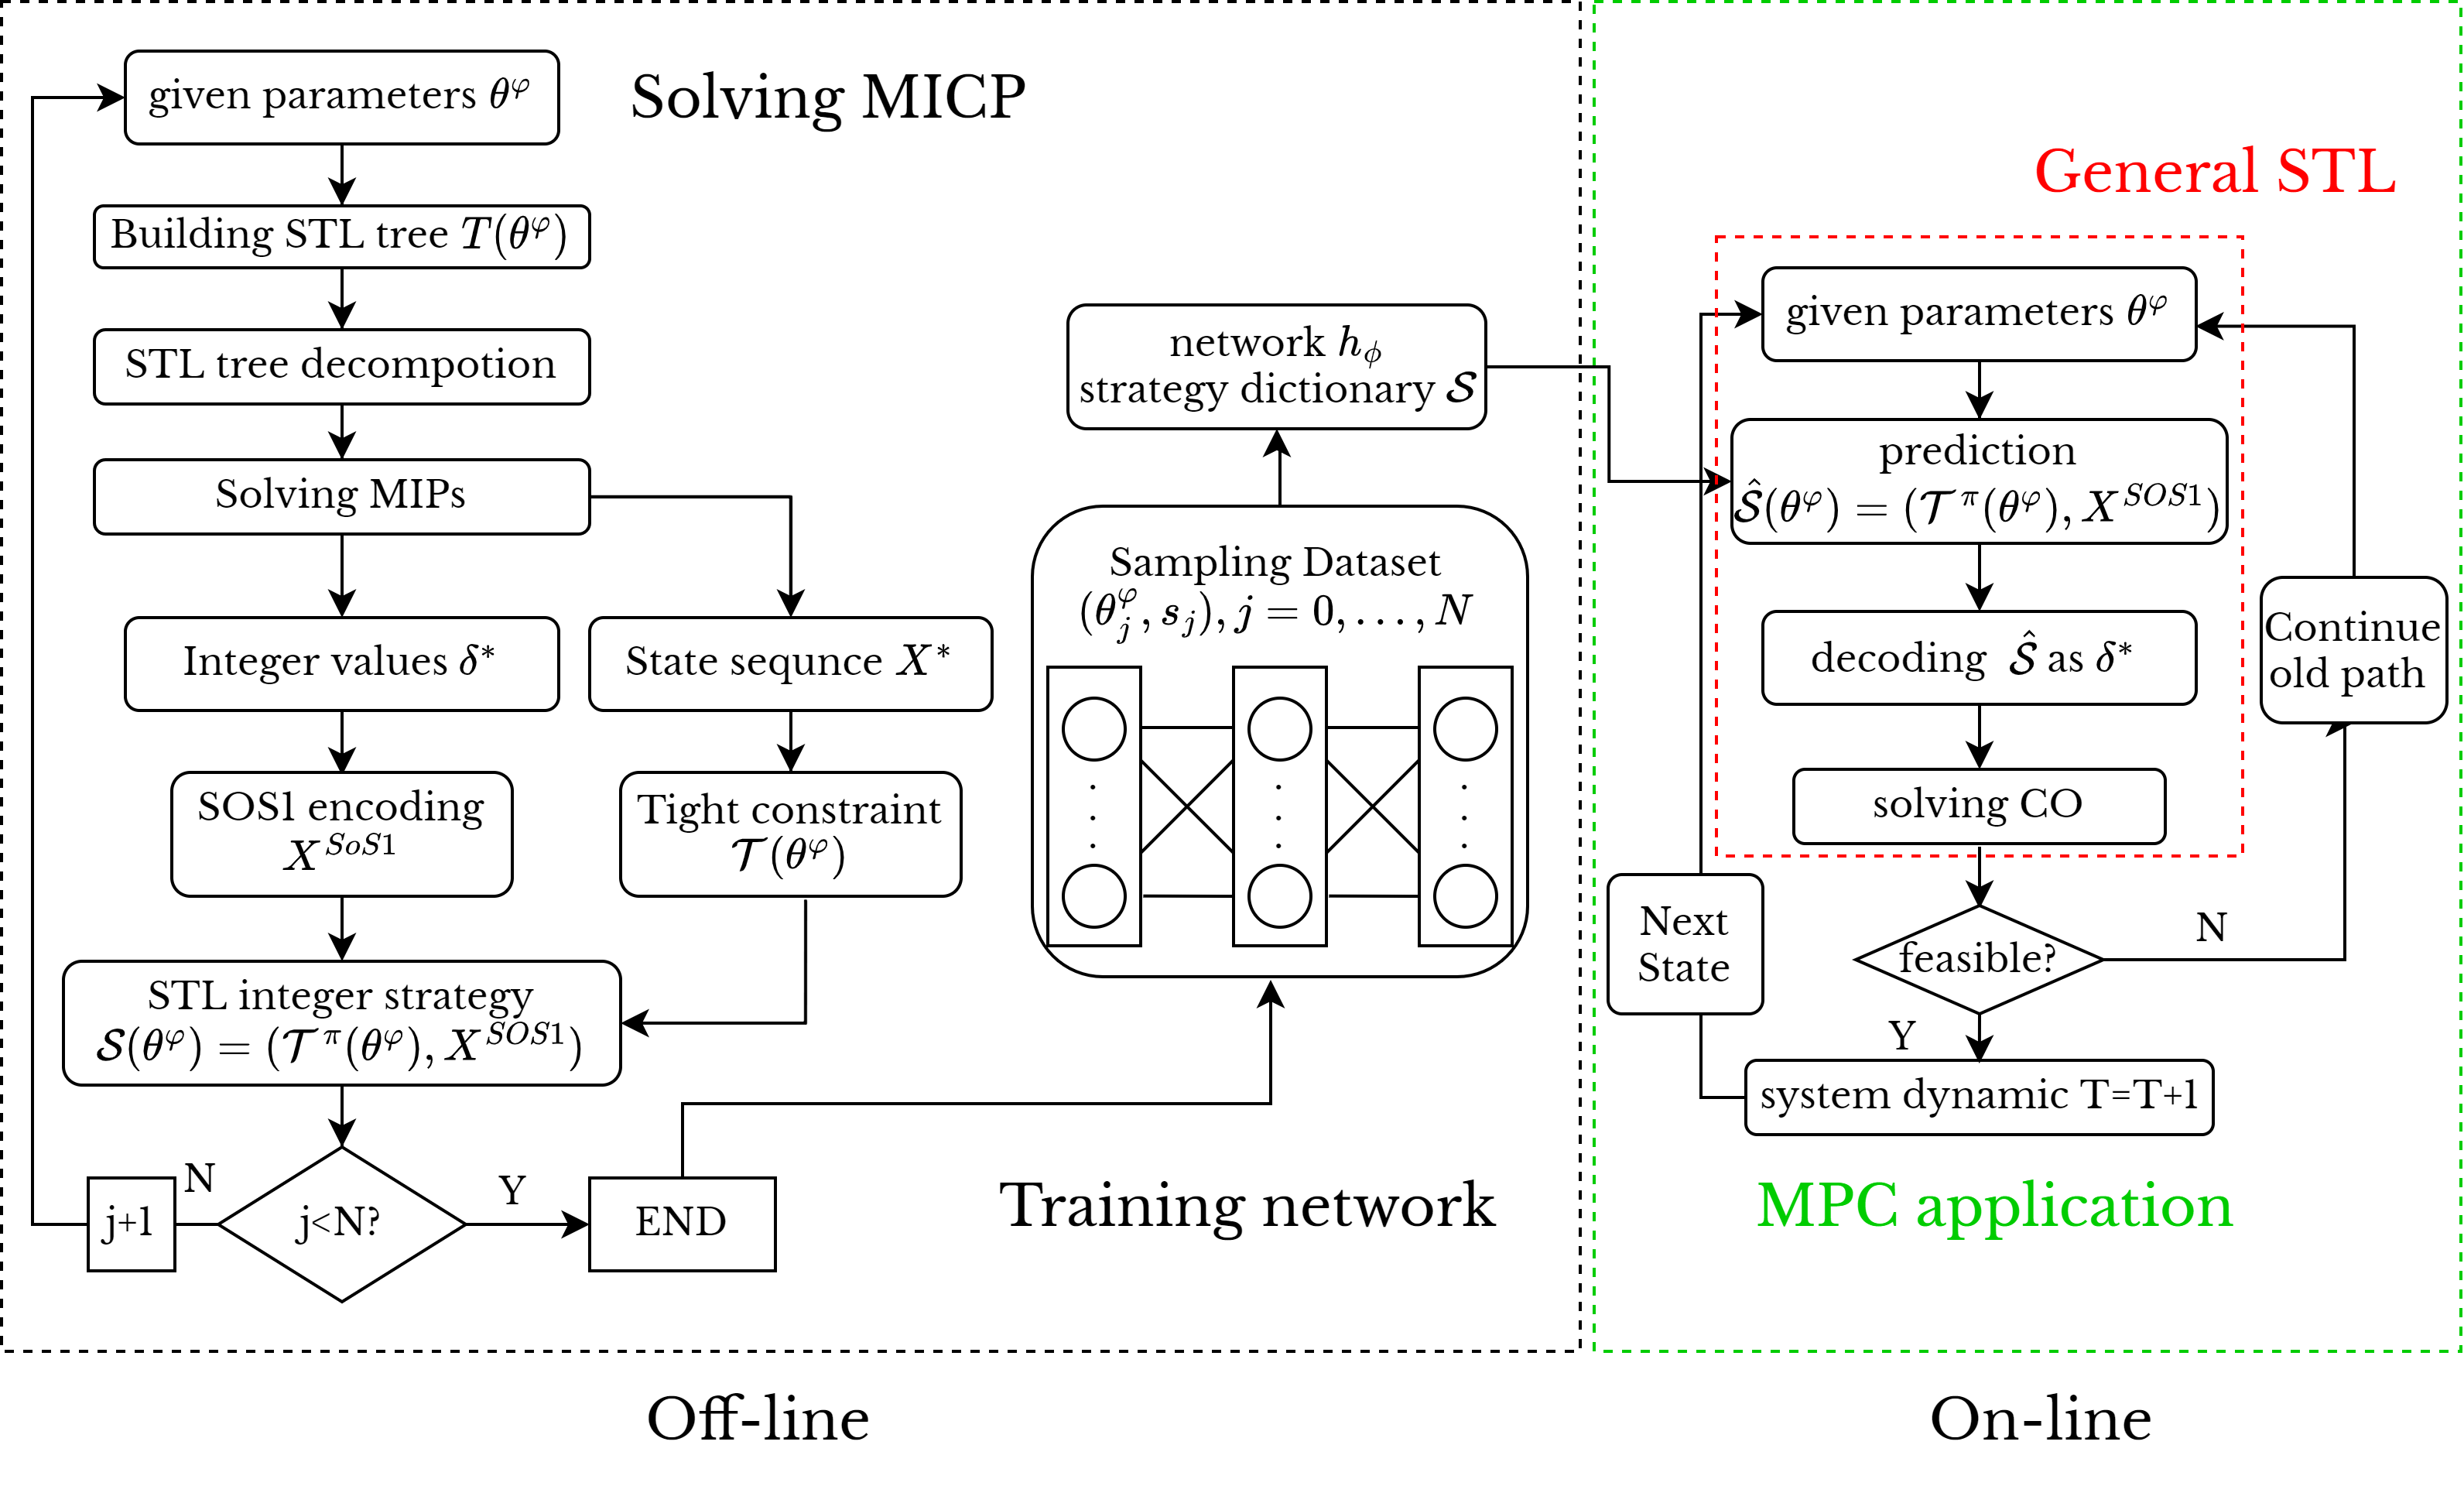
\includegraphics[scale=0.65]{omlstl.png}
    \caption{Framework of OMISTL}
\end{figure}

\section{STL tree structure} 
To propose a more efficient encoding for STL formula, here we apply the tree data structure as in \cite{kurtz2022mixed} \cite[]{leung2020back}. The tree data structure is formally defined as follows:
\begin{myDef} STL Tree structure. An STL tree $ E^\varphi$ is a tuple $(C, \tau, o , \rho^\varphi)$, where: \\
    1) $C = [E^\varphi_1,E^\varphi_2,...,E^\varphi_N]  $ is a list of $N$ subtrees (i.e., children) associated with each subformula;\\
    2) $\tau = [t^\varphi_1,t^\varphi_2,...,t^\varphi_N] $is a list of time stepscorresponding to the $N$ subformulas;\\
    3) $o \in \{ \wedge, \vee\}$ is the ombination type;\\
    4) $\rho^\varphi$ is the STL robustness measure: a function which maps signals $mathbb{y}$ to scalar values.
\end{myDef}

All nodes in an STL Tree are themselves STL Trees and correspond to subformulas. Leaves of an STL Tree correspond to predicates $\pi$.
For a given STL formula $\varphi$, a corresponding tree $E^\varphi$ can be built up recursively by following the syntax presented in formulas \ref*{robustness definition}.

For example, consider the specification $\varphi = \square_{[1,T]}a \wedge \Diamond_{[1,T]}b$, where $a$ and $b$ are predicates. The associated STL Tree is shown in Fig \ref{STLtree_simple}. There are two $\wedge$-type nodes (associated with $\varphi$ and $\square a$) denoted by the hollow circles, and one $\vee$-type node ($\Diamond b$) denoted by the solid circle, and 2T predicates denoted by the small triangles.

\begin{figure}
    \vspace{0.5cm}
    \centering
    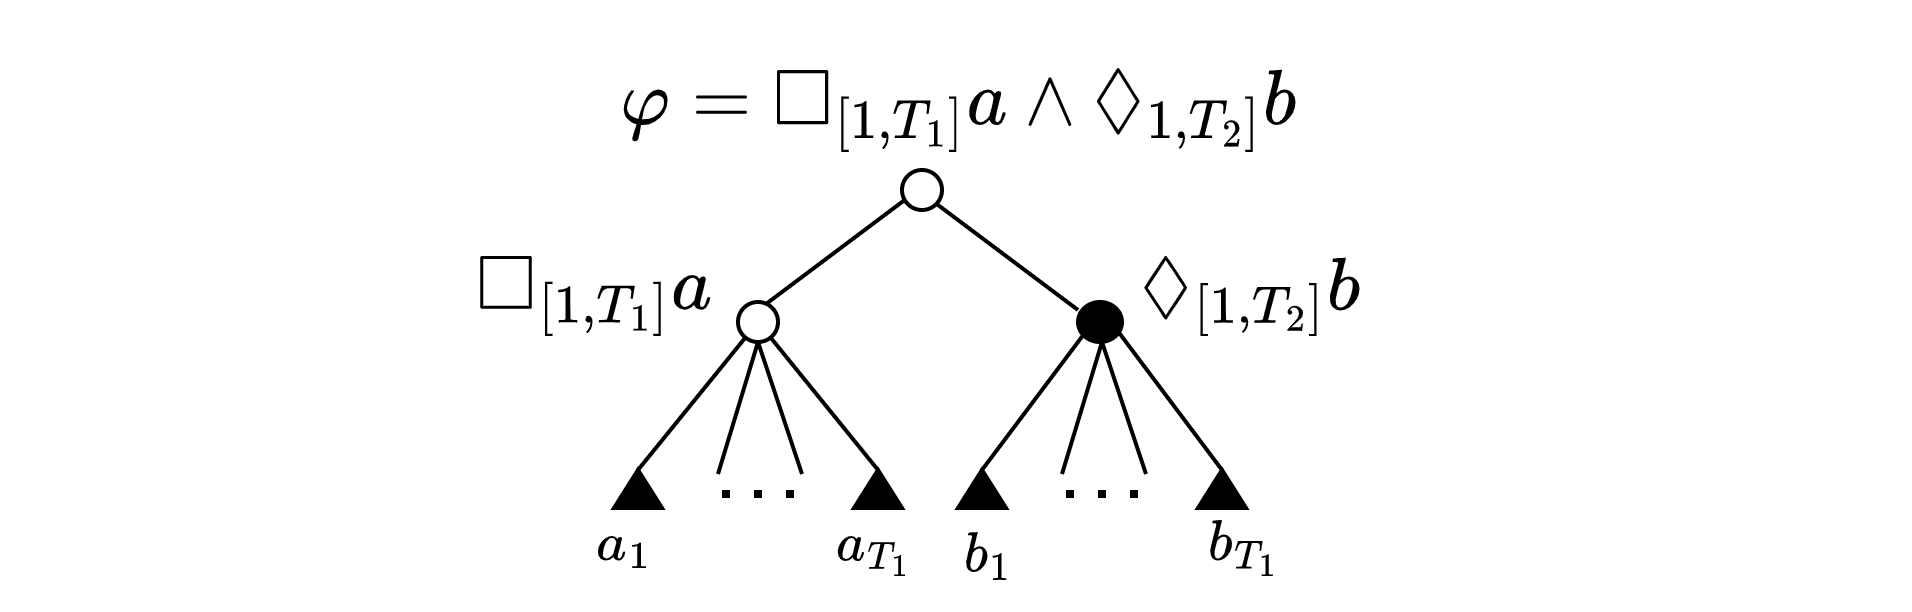
\includegraphics[scale=0.8]{STLtree_simple.png}
    \vspace{-0.4cm}
    \caption{STL tree structure of formula $\Box_{[1,T_1]}a\wedge \Diamond_{[1,T_2]}b$}
    \label{STLtree_simple}
    \vspace{-0.6cm}
\end{figure}

With the STL tree structure, we can encode the STL formulas as mixed-integer constraints with $\sum_{1}^{N^\lor}(\log_2(N_i+1))$ integer variables compared with the standard $TN^{\pi}$ in \cite[]{raman2014model}, where $N^\vee$ is the number of disjunctive formulas, $N_i$ is the number of subformulas for the $i_{th}$ disjunctions, and $N_{\pi}$ is the number of predicates. Note that $N_i$ may vary with the time horizon T depending on the specification. 

In an STL subtree that represents a disjunctive formula, we need to introduce one binary for the parent node and $N_i$ binaries for the children nodes. Thus for each disjunctive formula, $N_i+1$ binaries are required. Surprisingly, this number can be reduced further with a simple STL tree with only two layers. Because the binary variables represent whether the parent nodes hold or not, when the parent nodes are combined with the 'AND' relation, we can list the constraints together without introducing the parent node. In this particular scenario, the number of binary variables for each disjunctive formula can be reduced from $N_i+1$ to $N_i$. For instance, in the obstacle avoidance MPC problem, we reduce the typical $n\cdot T\cdot N_f$ to $n\cdot T\cdot \log_2N_f$ rather than $n\cdot T\cdot \log_2(N_f+1)$. This encoding approach will be present in section \ref*{Decomposition for MPC}, 

\section{Efficient STL encoding}

In this section, we will present how to implement our proposed efficient STL encoding.

Firstly, build the STL tree $E^\varphi$ from the given specification $\varphi$ and flatten the formula. Secondly, starting from the top node, we decompose the STL tree as $\wedge $-type nodes and $\vee$-type nodes until reaching the leaf nodes. For for each $\vee$-type node, we introduce $\log_2(N_i+1)$ integer variables and set SOS1 constraints, where $N_i$ is the number of subformula of the $i_{th}$ $\vee$-type node, 
the adding integer variables $\delta^\varphi_i$ is recorded as SOS1 encoding. Note that if we meet similar $\vee$-type nodes that are subnodes of a $\wedge$-type node, i.e. they have repeated structure inside the red lines as shown in fig.\ref*{mpc_tree}, the SOS1 encoding can be decomposed further based on the number of subnodes. Finally, we encode the variables $\delta^\pi_i$ that belong to the $\vee$-type leaf nodes as SOS1 encoding. Notably, no binary variable is introduced for the $\wedge$-type leaf nodes, and we only record the binary values from the $\vee$-type nodes because computing them is the bottleneck when soving MICPs. The specific procedure is present in fig.\ref*{stl_tree_decomposition}.

\begin{figure}[htbp] \centering 
    \vspace{0.5cm}
    \centering
    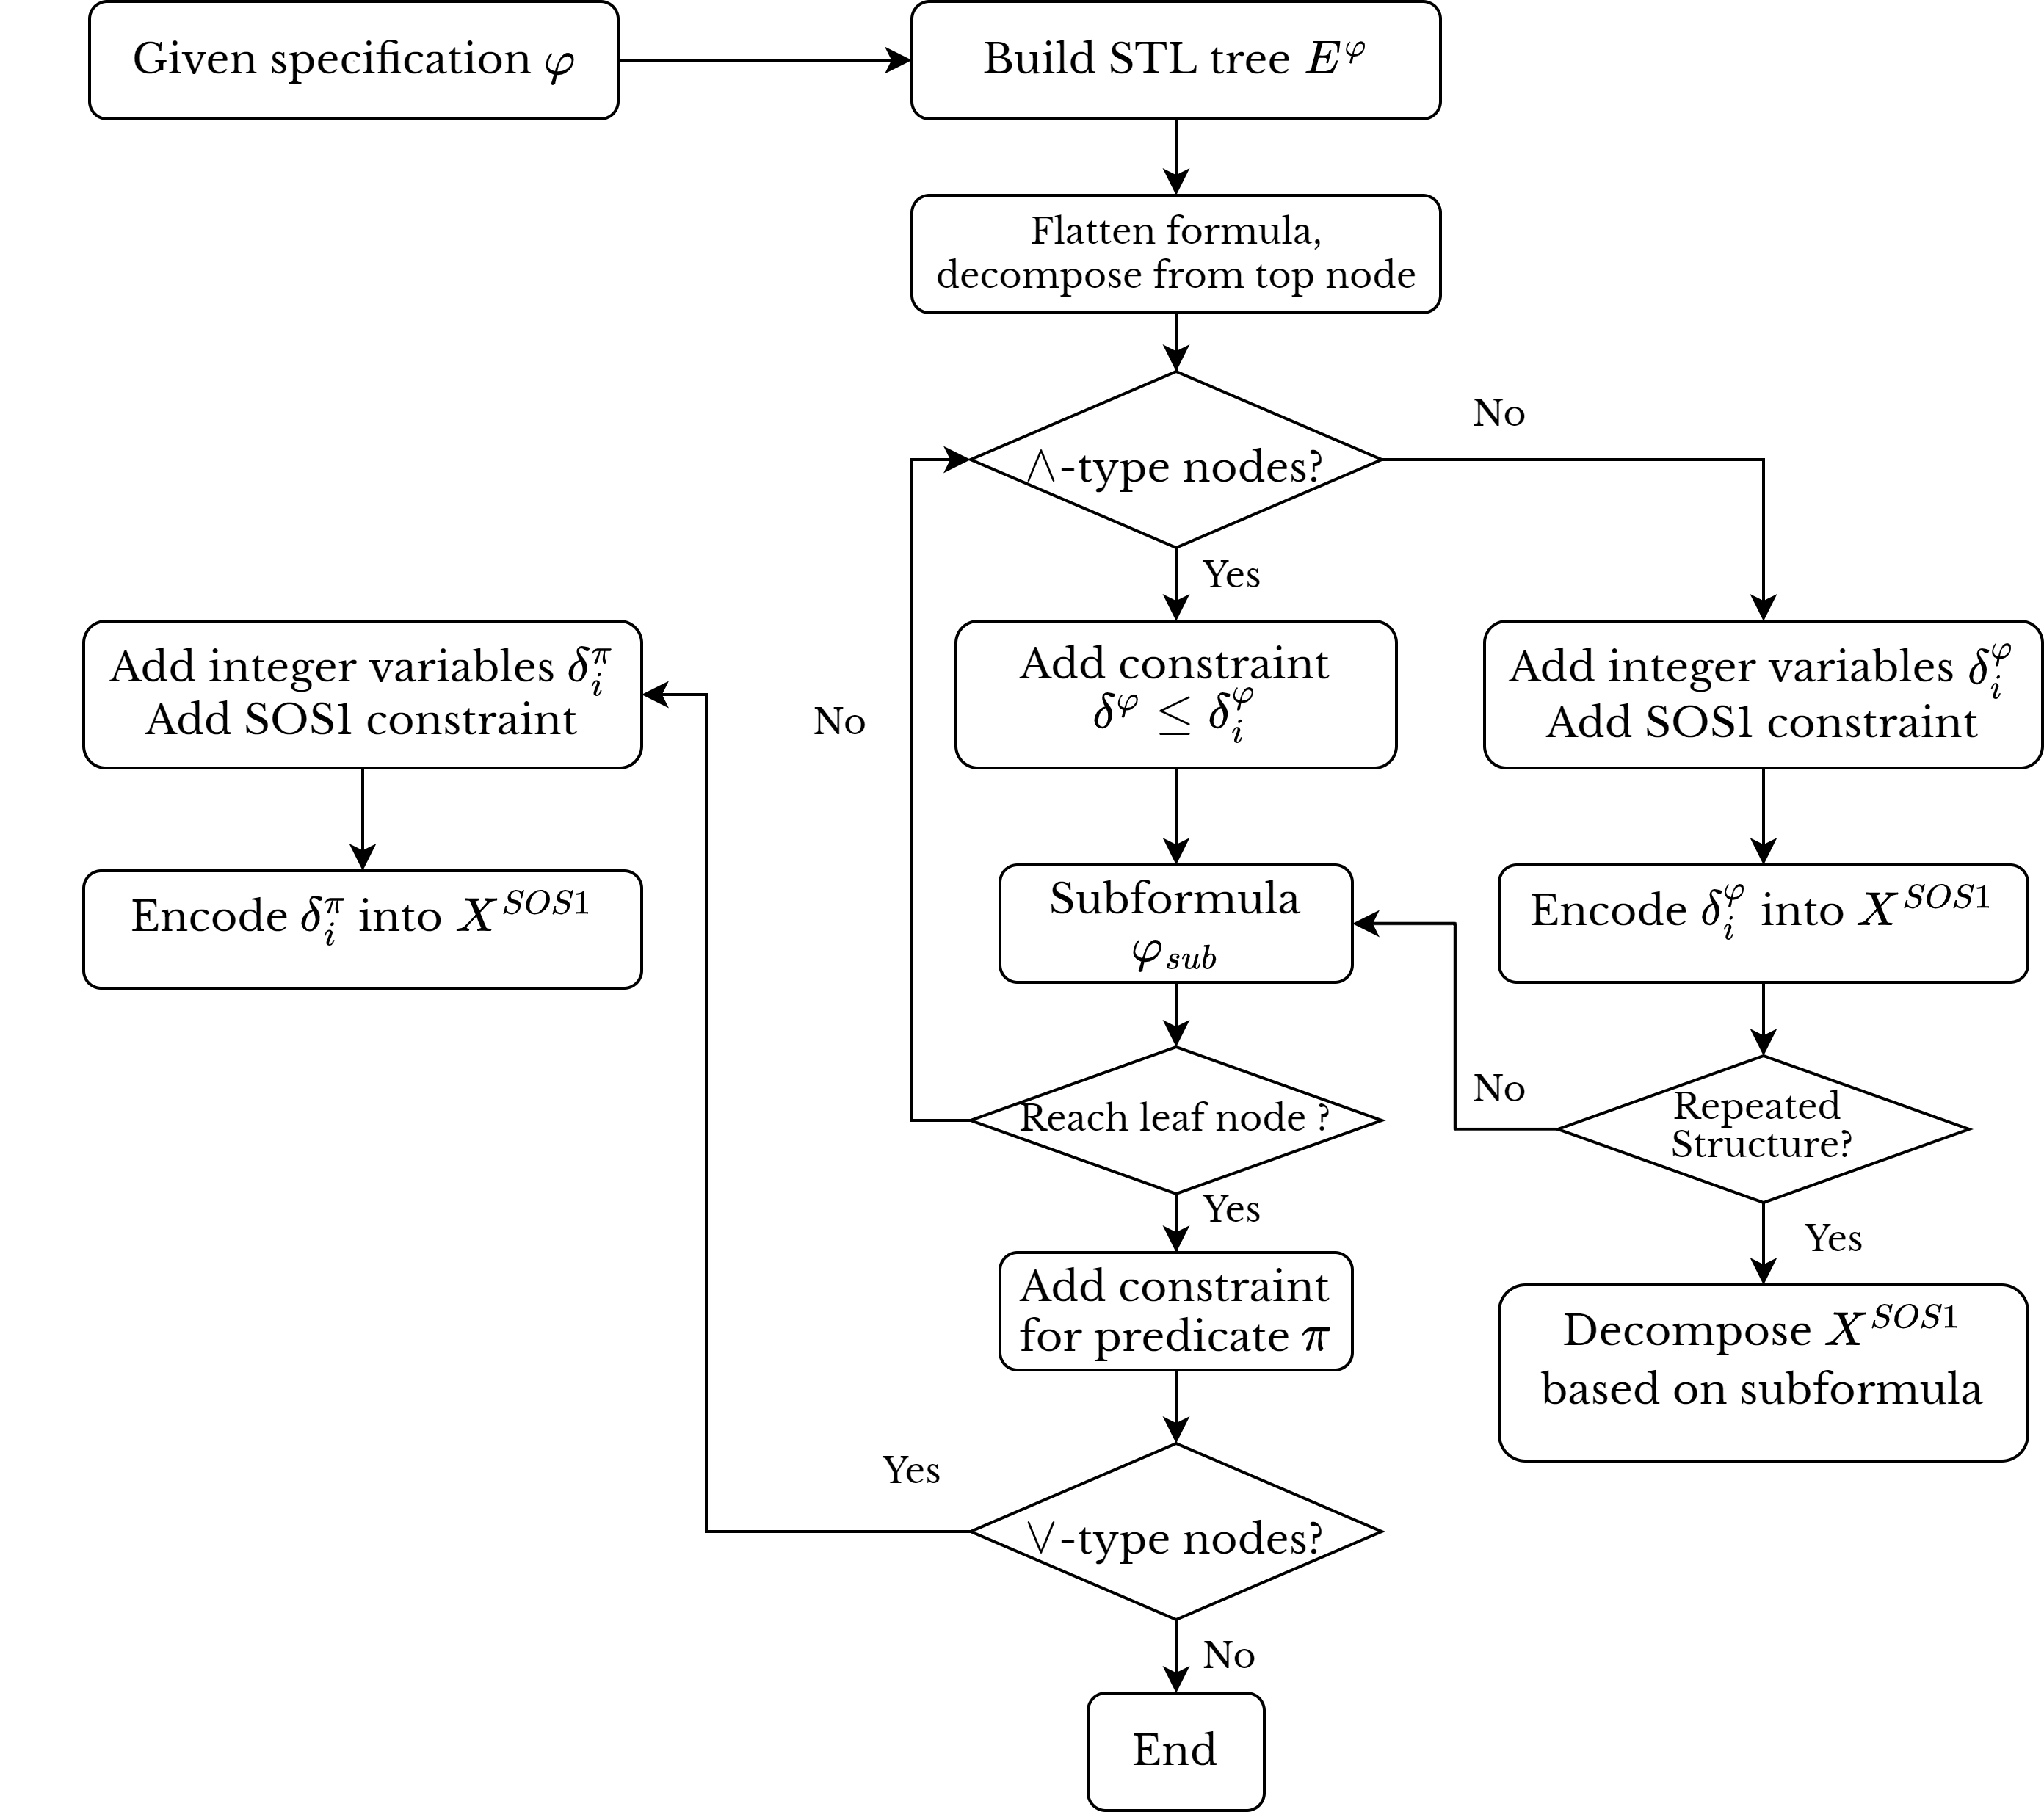
\includegraphics[scale=0.55]{stl_tree_decomposition.png}
    \caption{Efficient STL encoding}
    \label{stl_tree_decomposition}

\end{figure} 

\subsection{STL tree decomposition and SOS1 encoding}
\label{STL_encooding}
We specify now how to decompose the STL tree structure and formulate the mixed-integer constraints with our proposed SOS1 encoding. Given an STL formula $\varphi$, construct a corresponding STL Tree $T^\varphi$. The lower bound on the robustness measure $\rho^\varphi$ is defined as a continuous variable $\rho\geq0$, a violation of this constraint will render the problem infeasible. For each node in the tree $T^\varphi$, we set a continuous variable $ \delta^\varphi \in [0,1]$, where $\delta^\varphi=1$ if the subformula $\varphi$ is enforced. Declaring them as continuous improves MICP efficiency though $\delta^\varphi$ takes binary values.

The STL tree can be decomposed as three class of nodes, the leaf nodes,  $\wedge $-type nodes and $\vee$-type nodes, denoted by solid circle, hollow circle and triangle in fig.\ref{STLtree_simple}. Since each leaf node is associated with a predicate ($\pi$) and a timestep t, we try to impose such a relation:
\begin{equation}
    \delta^\pi = 1 \rightarrow g^\pi(\boldsymbol{y}_t) \leq 0,
    \end{equation}
so the big-M constraint is set as:
\begin{equation}
    \label{sosconstraint1}
    g^\pi(\boldsymbol{y}_t) \leq M(1-\delta^\pi),
\end{equation}
the $\wedge $-type nodes can be easily encoded by setting constraint:
\begin{equation}
    \label{sosconstraint2}
    \delta^\varphi \leq  \delta^{\varphi}_i, \quad \forall i=1,...,N
\end{equation}
without adding more binary variables, because $\delta^\varphi = 1$ implies all the subformulas $\varphi_1, \varphi_2,..., \varphi_N $ must also hold. For the $\vee$-type nodes, we need to introduce the definition of the SOS1 sets.

\begin{myDef}
    A vector $\lambda = [\lambda_1,\lambda_2,...,\lambda_n]^T $ is a set Special Ordered Set of Type 1 (SOS1) if the following conditions hold:\\
    1) $\lambda_i \geq 0$\\
    2) $ \sum_{i} \lambda_i =1$\\
    3) $ \exists j \in [1,...,n] s.t. \lambda_j=1$\\
\end{myDef}
\vspace*{-0.5cm}
In short, a vector $\lambda$ is in SOS1 if it contains exactly one nonzero element, and that element is equal to 1. we can constrain $\lambda \in SOS1$ using a logarithmic number of binary variables and constraints:

\begin{myTheo}
    (\cite{vielma2011modeling}) Assume that $n$ is a power of 2. Let $I = 1,2,...,n $ and $B: I \rightarrow \{0,1\}^{\log_2(n)}$ be any bijecetive function. Then the following constraints enforce $\lambda \in$ SOS1:
    \begin{equation}
        \label{sosconstraint3}
        \begin{aligned}
            \lambda_i &\geq 0, \quad \sum_{i}\lambda_i = 1,\\
            \sum_{j \in J^{+}(k, B)} \lambda_{j} &\leq \zeta_{k},  \sum_{j \in J^{0}(k, B)}
            \lambda_{j} \leq\left(1-\zeta_{k}\right),\\
            \zeta_{k} \in\{0,1\}, \quad & \forall k \in\left[1,2, \ldots, \log _{2}(n)\right]     
        \end{aligned}
    \end{equation}
\end{myTheo}
where $J^{+}(k, B)=\{i \mid k \in \operatorname{supp}(B(i))\}, J^{0}(k, B)=\{i \mid k \notin$ $\operatorname{supp}(B(i))\}$, and $\operatorname{supp}(B(i))$ denotes the support of $B(i)$.
Thus the constraints $\delta^\varphi \implies \vee_{i=1}^{N}\delta^{\varphi}_i$ can be written as a SOS1 constraint $\left[1-\delta^{\varphi}, \delta^{\varphi_{1}}, \delta^{\phi_{2}}, \ldots, \delta^{\varphi_{N}}\right] \in S O S 1$. Then the Reflected Gray Code (RGC) \cite{vielma2011modeling} is used to encode the index of the non-zero element in SOS1 vector $\lambda$, which is denoted by the SOS1 encoding $X^{SOS1}$. In other word we use $\log_2(N+1)$ binaries to imply the original vector with size $N$, e.g. $X^{SOS1}= [1, 1, 0]$ which equals to 5 implies a SOS1 vector $\lambda=[0,0,0,0,1,0,0,0]$, where $N$=7.

Similar to the existing MICP encodings \cite[]{raman2014model}\cite[]{kurtz2022mixed}, this MICP is sound, complete, and globally optimal:

\begin{myTheo}
    (\cite{kurtz2022mixed})
    Sound and Complete. A dynamically feasible output signal $y$ is a solution to Problem \ref*{stl_eq} if and only if y is a solution that satisfies constraints [3.1-3.3].
\end{myTheo}

\begin{myTheo}
    (\cite{kurtz2022mixed})
    Globally Optimal: If Problem \ref*{stl_eq} is feasible, the solution satisfies constraints [3.1-3.3] is globally optimal.
\end{myTheo}

It frequently occurs that sets of $\vee$-type nodes are used to model repeated but spatially or temporally distinct, phenomena. For example, to realize obstacle avoidance at each time step, we need to use a conjunction of similar $\vee$-type nodes at different time, as shown in fig.\ref{mpc_tree} within the red lines. They can be further decomposed via the proposed decomposition method.
% \begin{figure}[htbp]
%     \centering
%     \begin{minipage}[t]{0.48\textwidth}
%     \centering
%     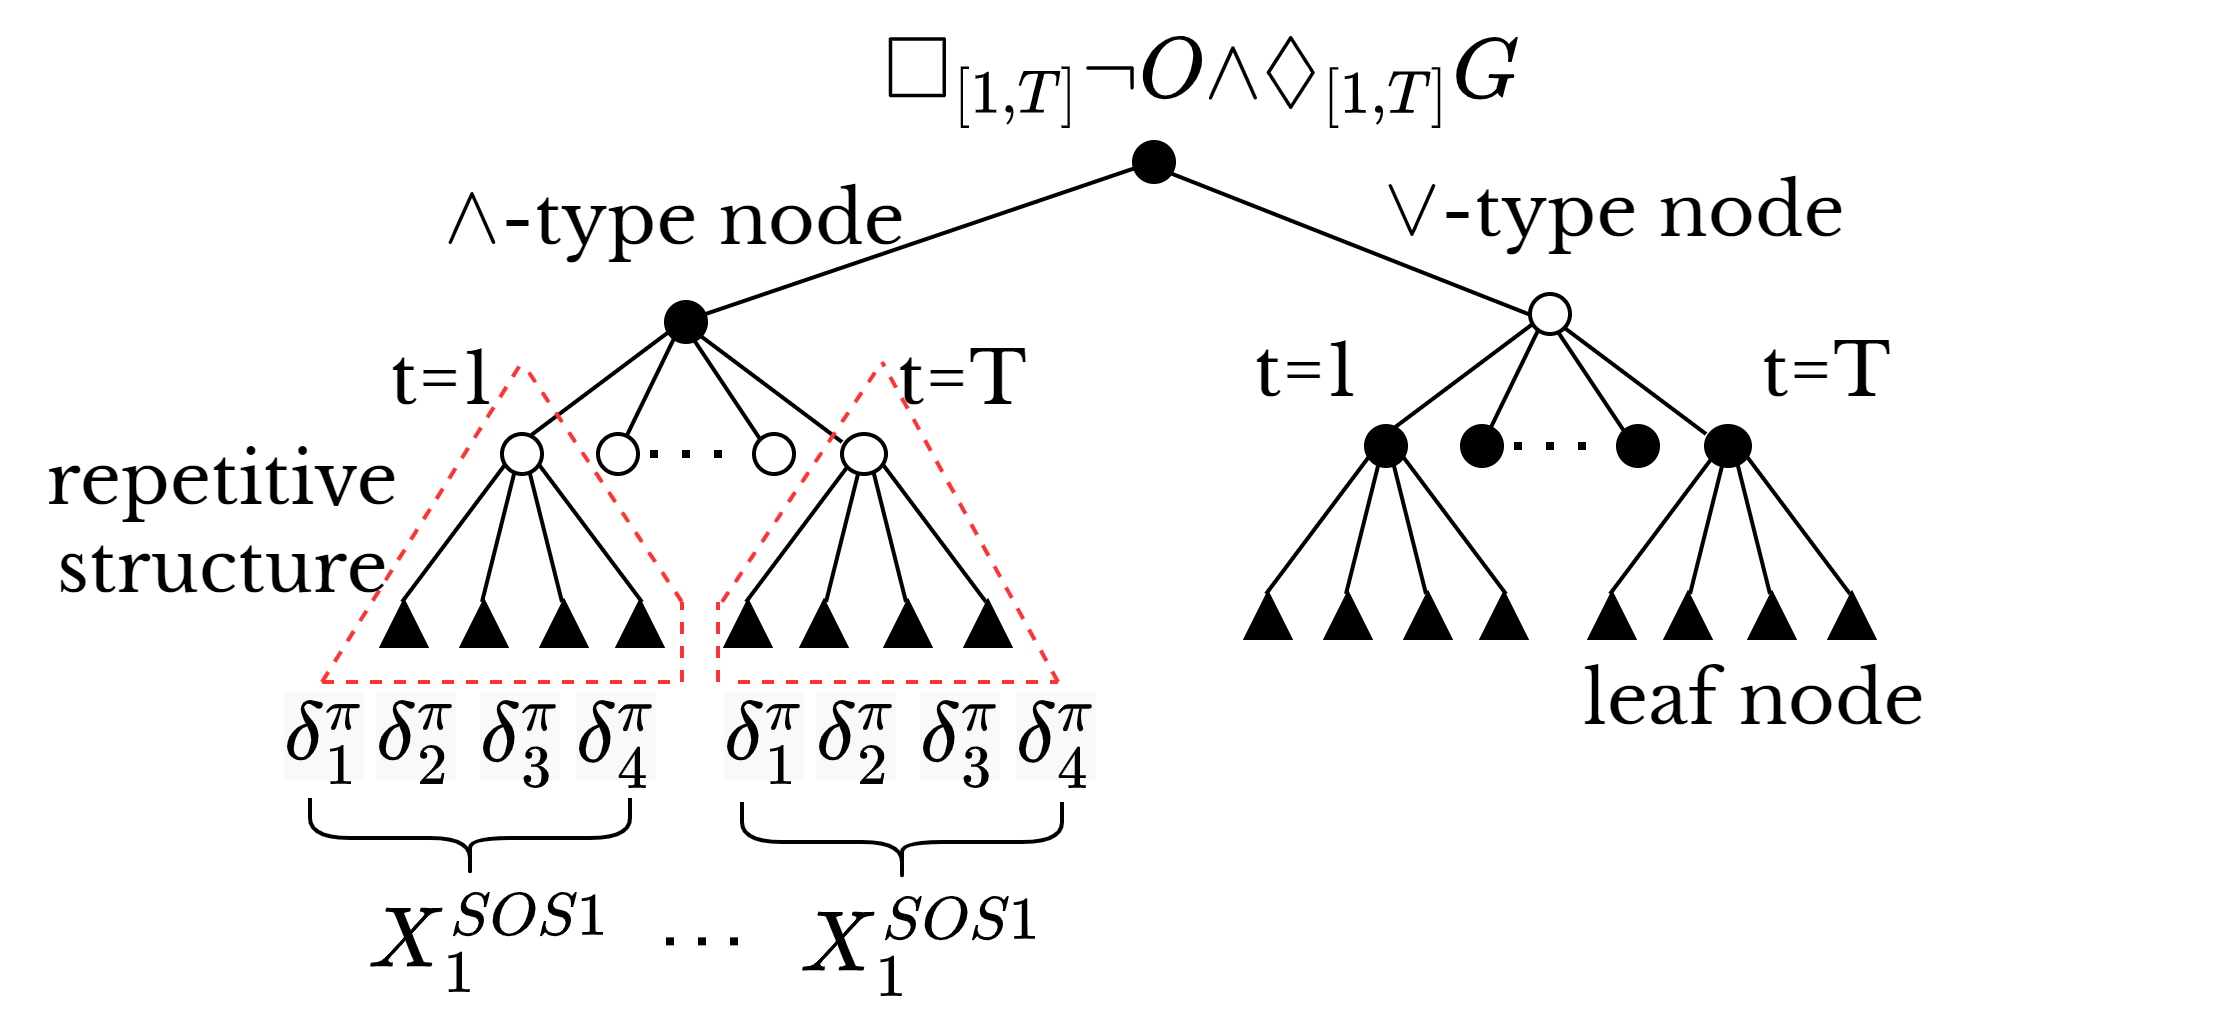
\includegraphics[width=6cm]{STL_tree.png}
%     \caption{STL Tree structure of $\Box_{[1,T]}a\wedge \Diamond_{[1,T]}b$}
%     \end{minipage}
%     \begin{minipage}[t]{0.48\textwidth}
%     \centering
%     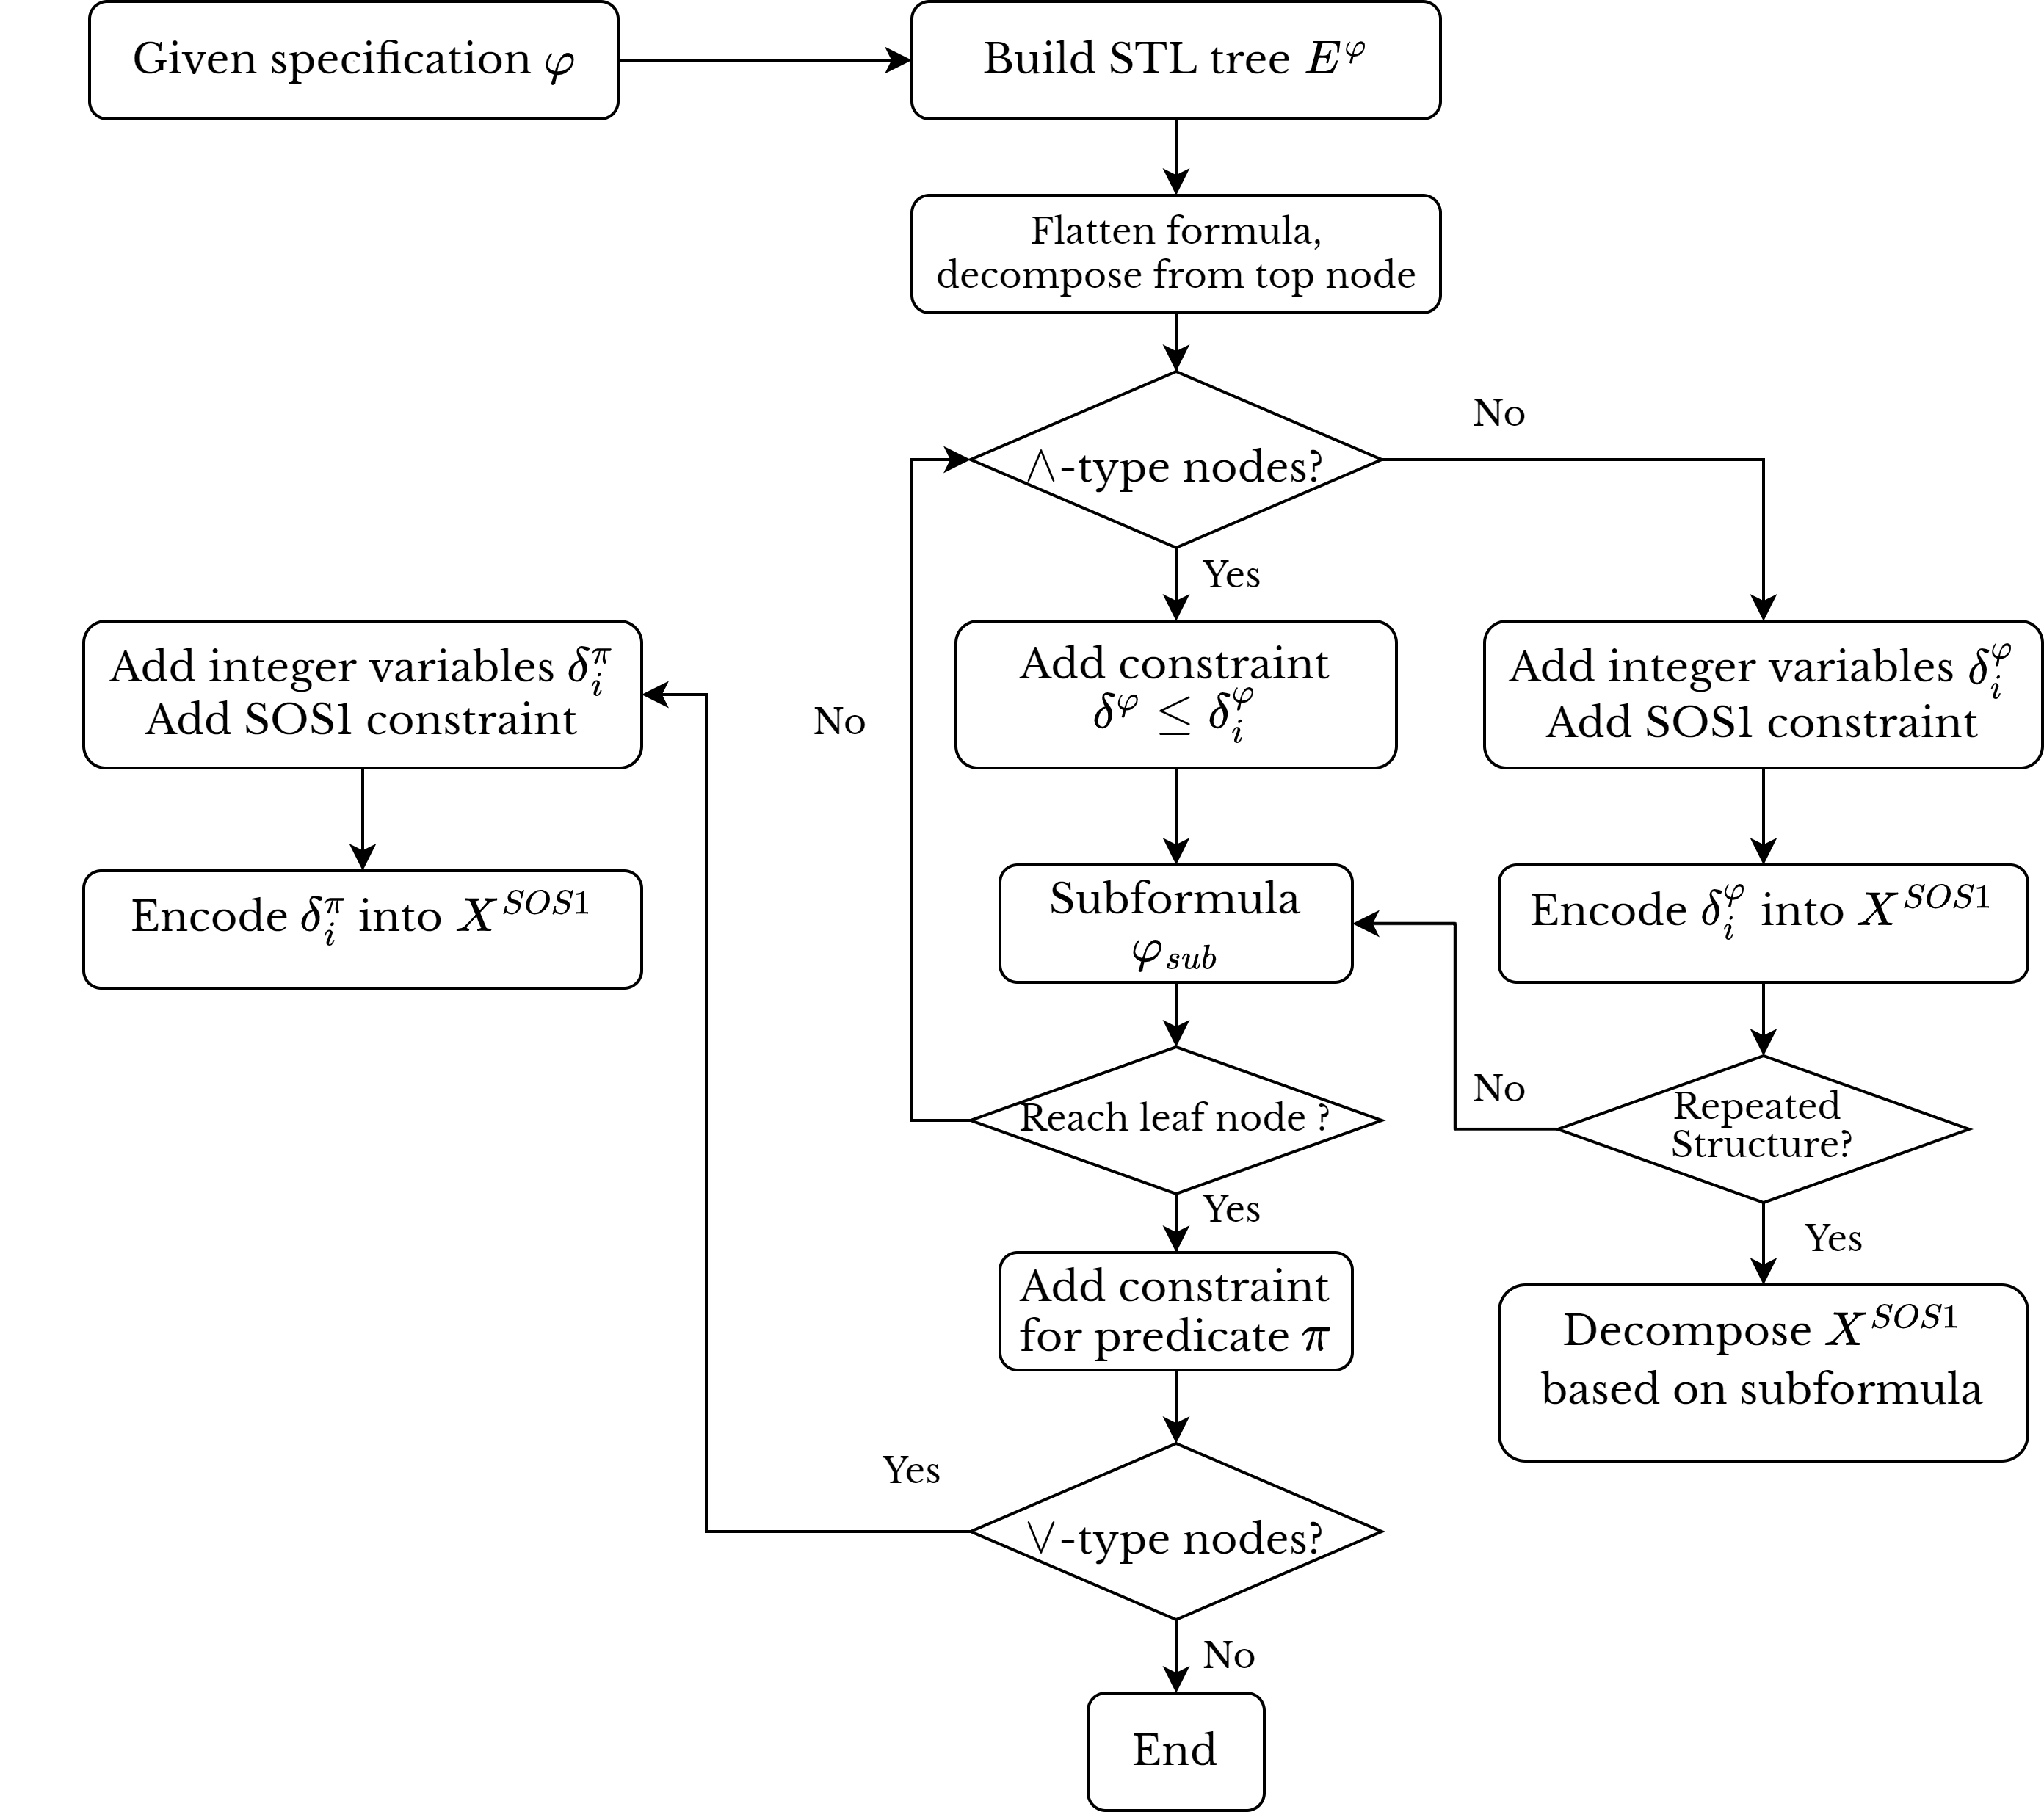
\includegraphics[scale=0.7]{stl_tree_decomposition.png}
%     \caption{STL tree decomposition method}
%     \end{minipage}
%     \end{figure}

While the method in \cite{kurtz2022mixed} only decomposes the specification as $\wedge $-type nodes and $\vee$-type nodes, our proposed method can further decompose these nodes with a repeated structure, including the predicate nodes, and an efficient SOS1 encoding is proposed to record the resulting STL tree strategies. The detailed procedure is shown in fig.\ref{stl_tree_decomposition}. According to the Theorem [1]-[3], this method is sound and complete, ensuring finding a globally optimal solution \cite[]{kurtz2022mixed}.

\subsection{Examples to illustrate the STL encoding} 

To illustrate our STL encoding and understrand how it differs from the tipical encoding, we present two simple expamles which only consider avoiding one obstacle at one timestep using the two encodings.

\subsubsection*{Typical STL encoding}

We present how to formulate the optimization problem based on the standard encoding. To start with, we require the state $x$ belongs to a “safe” set $\mathcal{X}$, denoted by $x \in \mathcal{X}$, which is equivalent to the obstacle avoidance specification $\lnot O$. Note that we ignore the time series to make it explicit. The set $\mathcal{X}$ consists of the area outside of a polyhedral obstacle with $N_f$ faces. Then, the set $\mathcal{X}$ can be written as:

\begin{equation}
    \mathcal{X}:= \{x \in \mathbb{R}^{n_x}:\bigvee_{j=1}^{N_f} a_j^Tx_ +b_j>0 \},
\end{equation}
by big-M method, we obtain the set describing the constraints on the state, and equivalently rewrite it as:
\begin{equation}
    \mathcal{X}:= \{x \in \mathbb{R}^{n_x}:\bigwedge_{j=1}^{N_f} a_j^Tx_ +b_j +M(1-\delta_j)>0 \},
\end{equation}
to formulate 'OR' relation we need at least one $\delta_j$ equal to 1, thus add constraint:
\begin{equation}
    \sum_{j=1}^{N_f} \delta_{j} \geq 1,
\end{equation}
putting the above developments together we can propose the optimization problem:
\begin{equation}
    \begin{aligned}
        \min \quad       &  J(x,u)\\
        \text{s.t.}\quad &
        x =x_o, u= u_o,                        
         \\
                         & a_1^Tx_ +b_1 +M(1-\delta_1)>0,                                   \\
                         & \cdots \\
                         & a_{N_f}^Tx + b_{N_f} +M(1-\delta_{N_f})>0,                                   \\
                         &    \sum_{j=1}^{N_f} \delta_{j} \geq 1, \delta_{j} \in \{0,1\},
    \end{aligned}
    \label{simple_ex1}
\end{equation}
the decision variables include continuous $x \in \mathbb{R}^{n_x}$, $u \in \mathbb{R}^{n_u}$, and the binary variables $\delta_j \in \{0,1\}$. Since we only focus on one timestep so the dynamic constraints are removed to simplify the problem. When $N_f=4$, 4 binary variables $\delta_j (j=0,1,2,3)$ and 5 constraints for big-M method are used for this problem.

\subsubsection{Our SOS1 encoding}

For SOS1 encoding we still use big-M method to formulate the "safe" set $\mathcal{X}:= \{x \in \mathbb{R}^{n_x}:\bigwedge_{j=1}^{N_f} a_j^Tx_ +b_j +M(1-\delta_j)>0 \}$ as the previous encoding, but constrain the binary variables $\delta_j$ in a different way.

Firstly, we declare all the binary variables $\delta_j$ as continuous and denoted by $\delta_j^c \in \mathbb{R}$:
\begin{equation}
    \delta_j^c \geq 0, \quad \sum_{j=1}^{N_f} \delta_{j}^c=1
\end{equation}
then assume that $N_f$ is a power of 2, let $ I=1,2,...,N_f $ and $B:I \rightarrow \{0, 1\}^{\log_2N_f}$ be any bijective function. If $N_f$ is not a power of 2, we can simply add $e^{\left\lceil\log _2 n\right\rceil}-n$ elements along with linear constraints $\delta_j=0$ that force these elements to be zero.

Now we introduce $\log_2N_f$ binary variables $\zeta_k \in\{0,1\}, \forall k \in\left[1,2, \ldots, \log _2(N_f)\right]$. Then add such constraints:

\begin{equation}
    \sum_{j \in J^{+}(k, B)} \lambda_j \leq \zeta_k, \sum_{j \in J^0(k, B)} \lambda_j \leq\left(1-\zeta_k\right)
\end{equation}
where $J^{+}(k, B)=\{i \mid k \in \operatorname{supp}(B(i))\}, J^0(k, B)=\{i \mid k \notin$ $\operatorname{supp}(B(i))\}$, and $\operatorname{supp}(B(i))$ denotes the support of $B(i)$.
With these constraints we can force the continuous vector $[\delta_1^c,\delta_2^c,...,\delta_{N_f}^c]$
to be a SOS1 vector that only contains one nonzero element and others are zeros.

Integrated with the SOS1 constraints, to make it clear we set $N_f = 4$ and the optimization problem \ref{simple_ex1} can be rewritten as:
\begin{equation}
    \begin{aligned}
        \min \quad       &  J(x,u)\\
        \text{s.t.}\quad &
        x =x_o, u= u_o                        
         \\
                         & a_1^Tx +b_1 +M(1-\delta_1^c)>0                         \\
                         & \cdots \\
                         & a_4^Tx +b_4 +M(1-\delta_4^c)>0                         \\
                         & \delta_0^c+ \delta_1^c+\delta_2^c+\delta_3^c =1
                         \\
                         & \delta_2^c+ \delta_3^c \leq \zeta_0
                         \\
                         & \delta_2^c+ \delta_3^c \leq 1-\zeta_0
                         \\& \delta_1^c+ \delta_2^c \leq \zeta_1
                         \\& \delta_1^c+ \delta_2^c \leq 1-\zeta_1
                         \\& \delta_j^c \geq 0; \quad \zeta_k \in \{0,1\}
    \end{aligned}
\end{equation}
the decision variables include continuous $x \in \mathbb{R}^{n_x}$, $u \in \mathbb{R}^{n_u}$, $\delta_j^c \in \mathbb{R}$ , and the binary variables $\zeta_k \in \{0,1\}$. Compared with the the encoding in \ref{simple_ex1}, SOS1 encoding uses only 2 binary variables $\zeta_j (j=0,1)$ but have more constraints and continuous variables for this problem.

This obstacle avoidance encoding consists of only an 'OR' logical relation. For more complicated scenarios, we need to combine the STL tree structure with the SOS1 encoding to impose the constraints.

\section{Model-predictive controller}
\subsection{ STL tree decomposition for MPC}
\label{Decomposition for MPC}

Thanks to our STL tree decomposition method, this specification can be formulated with a logarithmic number of binary variables, rendering the STL integer strategy in a more concise form compared with \cite{bertsimas2022online}\cite{Cauligi2020}. Since the obstacle avoiding specification can be represented as a conjunction of $\Box_{[0,T]}\lnot O_i(i=1,...,n)$, where $n$ is the number of obstacles and $\lnot O_i$ is a distinct sub-formula encoding that the robot must lie outside a single obstacle $i$:
\begin{equation}
    \Box_{[0,...,T]}(\bigwedge_{i=1}^n\lnot O_i) \Rightarrow (\Box_{[0,T]}\lnot O_1 \wedge \Box_{[0,T]}\lnot O_2\wedge...\wedge \Box_{[0,T]}\lnot O_n),
\end{equation}
An interesting observation is that the subformulas sometimes have similar structures as shown in fig.\ref{mpc_tree} (the subtree in the red dotted line), and each subtree refers to a set of disjunctive subformulas, i.e. always avoiding one obstacle. Leveraging this insight, we can decompose $\varphi$ on a per-obstacle basis, thus the resulting strategies can be decomposed into the sub-formula strategies $\mathcal{S}(\theta^\varphi) = \mathcal{S}_1(\theta^\varphi), \mathcal{S}_2(\theta^\varphi),...,\mathcal{S}_n(\theta^\varphi)$. 

\begin{figure}
    \vspace{0.5cm}
    \centering
    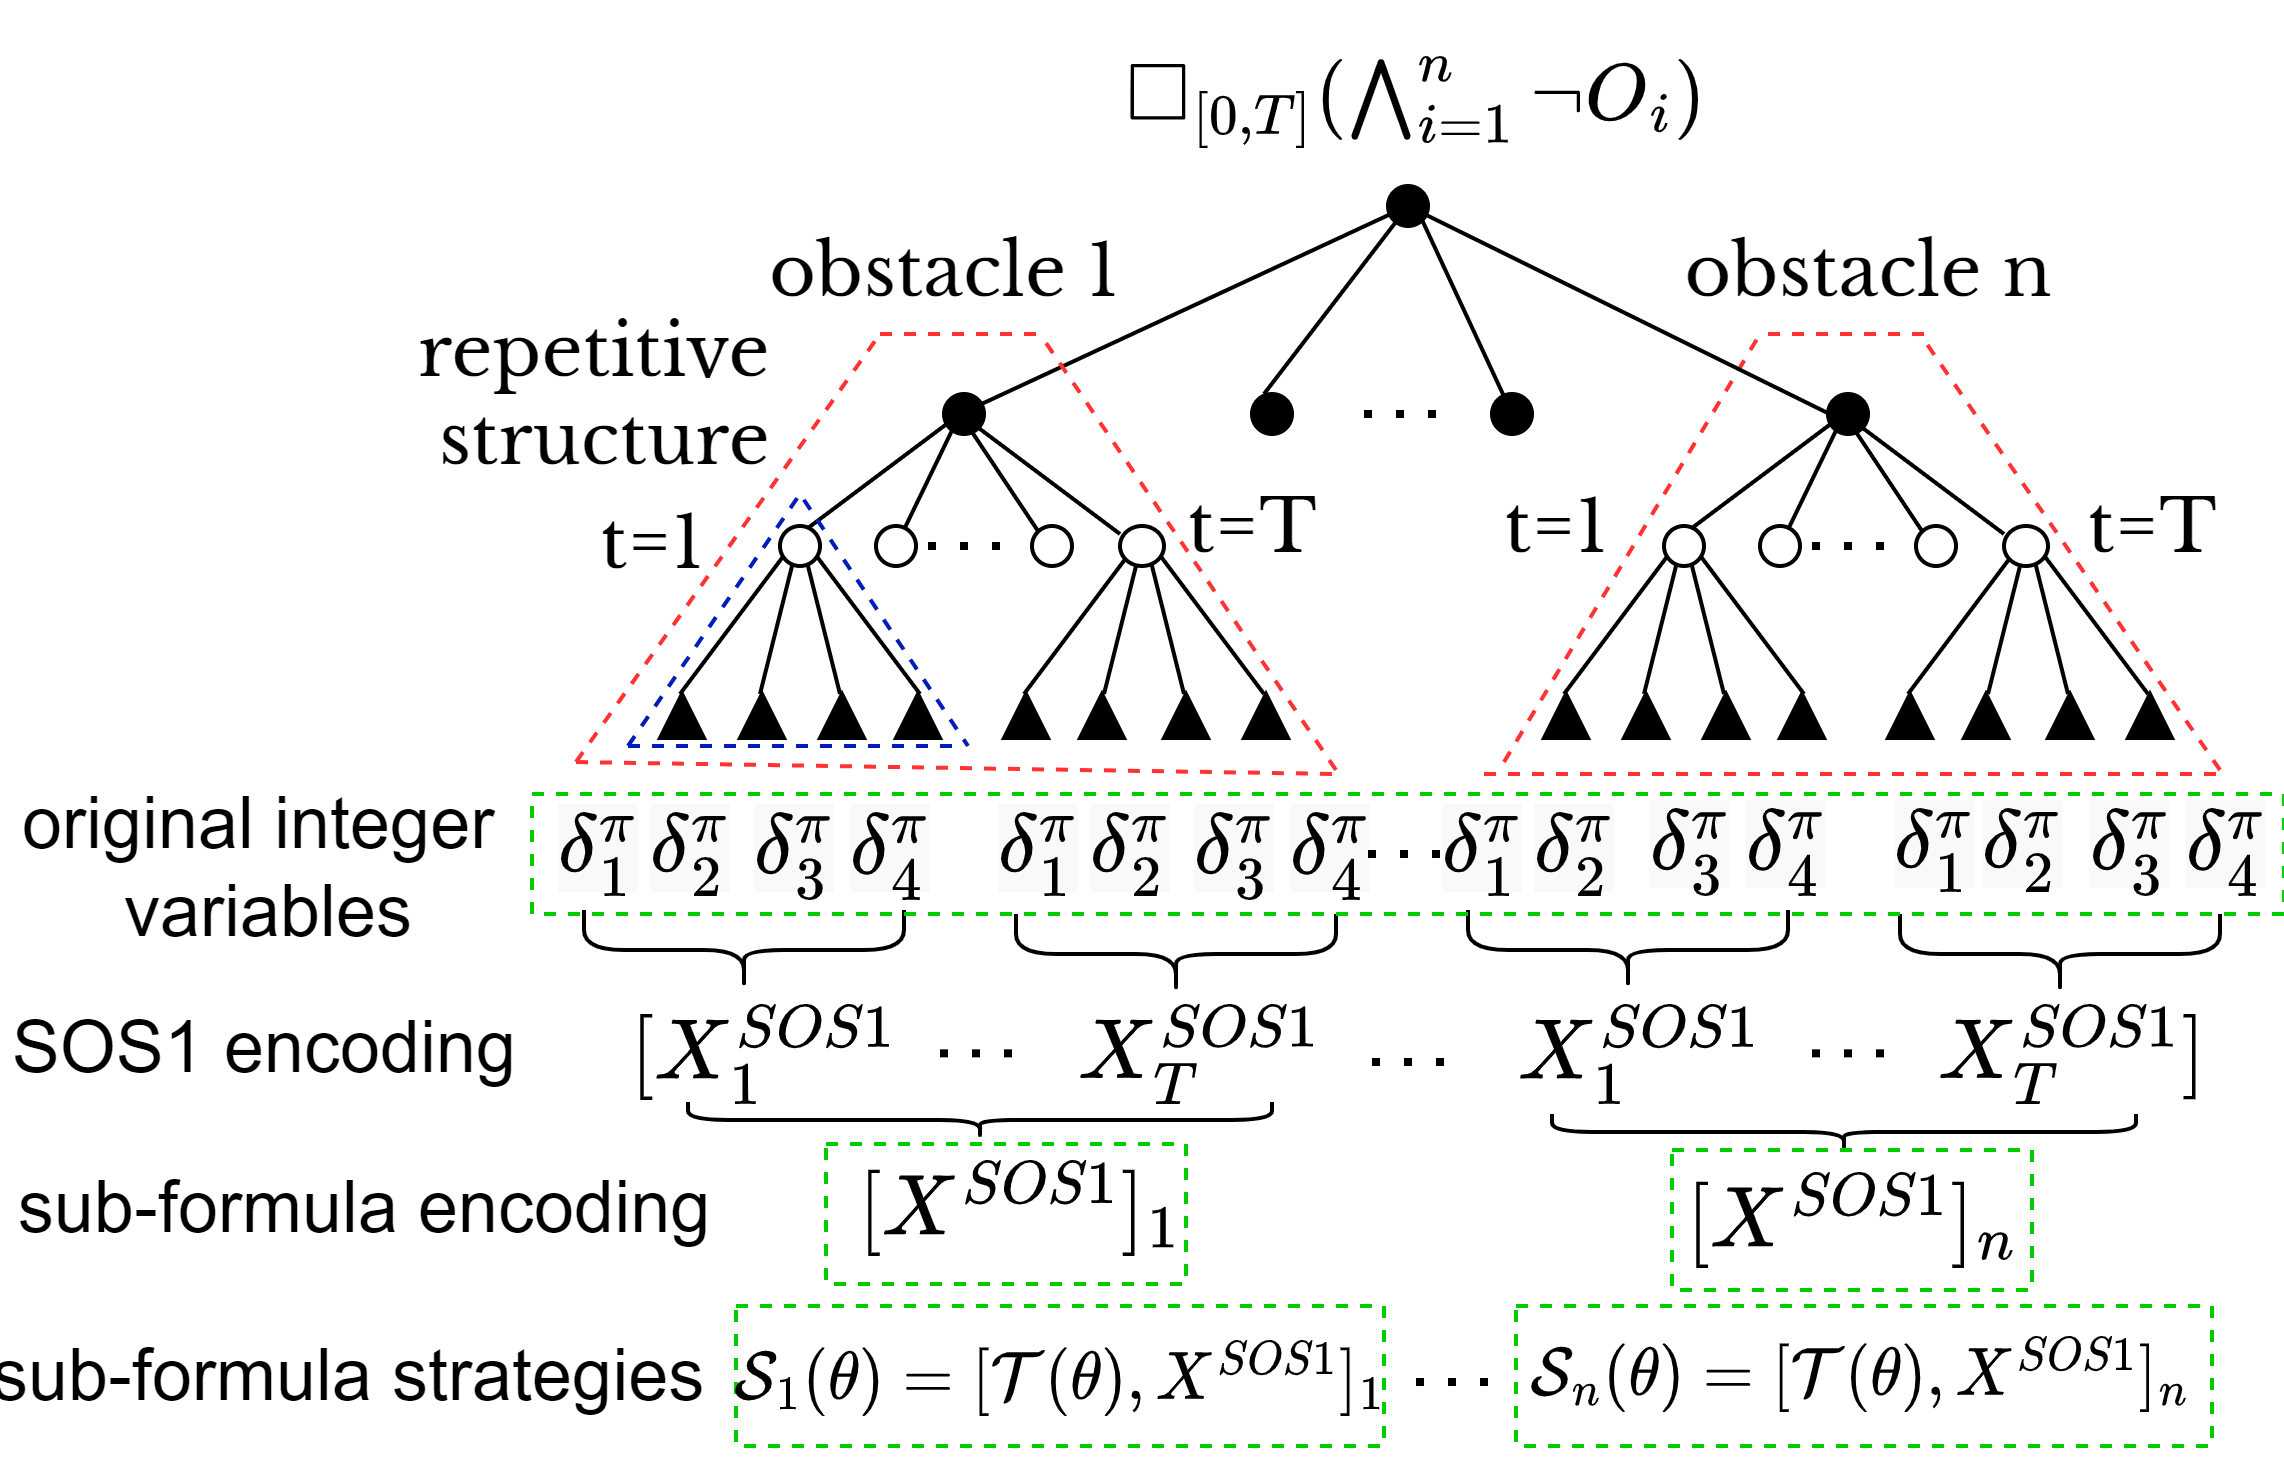
\includegraphics[scale=0.7]{mpc_tree.png}
    \vspace{-0.4cm}
    \caption{Decomposition and sub-formula strategy encoding for MPC }
    \label{mpc_tree}
    \vspace{-0.5cm}
    \end{figure}

\subsection{Strategy encoding and feature vector}
\label{Strategy encoding and feature vector}

As shown in fig.\ref{mpc_tree}, we take the sub-formula strategy $\mathcal{S}_i(\theta^\varphi)$ as the STL integer strategy, which is more succinct with $T\log_2(N_f+1)$ dimension rather than $nT\log_2(N_f+1)$ in contrast to without decomposition. Decomposing $\varphi$ into subformulas reduces the number of resulting strategies, since the subformulas may apply the same binary values due to similar structures. Surprisingly, since all the parent nodes of each obstacle are combined with an 'AND' relation, we can remove the parent node and list all the constraints together, which is equivalent to formulating the 'AND' relation. In this way, only $T\log_2N_f$ binaries are required, which further reduces the number. 
 
For instance, let $N_f =4$ as in fig.\ref*{mpc_tree}, four binary variables $\delta_i^{\pi}$ are required for constraining the robot to stay on one side among four faces for a rectangle obstacle \cite{bertsimas2022online}\cite{Cauligi2020}. Due to the repetitive structure of the variables $\delta_i^{\pi}$ used for each predicate $\pi$ (the blue dotted line in \ref{mpc_tree}), we can use the SOS1 encoding $X^{SOS1} \in \{0,1\}^{Tlog_2N_f}$ to substitute the original $\delta_{i}^{\pi} \in \{0,1\}^{TN_f}$ with fewer binary variables. The number of binary variables used for this specification can be reduced from $nT\cdot N_f$ to $nT\cdot \log_2N_f$ where $N_f=4$ is the number of obstacle faces in this problem.

Although decomposing $\mathcal{S}(\theta^\varphi)$ into $n$ subformula strategies deduces the complexity and the number of the strategies, it leads to $n$ more classification tasks. Rather than training $n$ separate strategy classifiers for each $\mathcal{S}_i(\theta^\varphi)$, we train a single classifier using $\theta^\varphi$ and a one-hot vector of size $n$ to encode the index of each obstacle strategy. The insight behind it is that we take the parent node position of the sub-strategy as the classification feature, where the one-hot vector $X^{oh}$ is the index of obstacles, which also represents the index of the parent node to be attached, refer to the solid circle in fig.\ref{mpc_tree}. Therefore, after training the network "remembers" which parent node the sub-strategy should be attached to in the STL tree. After prediction the network will return $n$ independent substrategies corresponding to different obstacles, with the index information, one can recovered the original non-decomposed strategy and use it to solve the reduced problem. 

This approach can not only deal with avoiding multiple obstacles, but also be extended into more general cases, where the conjunctive $\vee$-type nodes with similar structure appears repeatedly in the STL tree, we can decompose the strategy as sub-strategies and use the one-hot vector to denote each parent node.

For MPC the input feature vector (i.e. the parameter $\theta^\varphi$) consists of the initial and final states $(x_0,v_0,x^{ref},x^{ref}) \in \mathbb{R}^8$, coordinates of each obstacle $X_i^o=(x_{i}^{min},x_{i}^{max},y_{i}^{min},y_{i}^{max}) \in \mathbb{R}^4$ where $i \in{1,...,n}$ and a one-hot code $X^{oh} \in \mathbb{R}^n$. After decomposition the $j_{th} $ data point $(\theta_j^{\varphi}, s_j)$ will result in $n$ feature vectors and labels, the vector $\theta_{i,j}^{\varphi} = [x_0,v_0,x_g,v_g,X_1^o,...,X_n^o,X_i^{oh}]$ where $X_i^{oh}$ is the one-hot vector of obstacles $i$, and the label $s_j$ is index of the STL integer strategy $\mathcal{S}_{i,j}(\theta^{\varphi})= [\mathcal{T}^{\pi}(\theta_{i,j}^{\varphi}), X_{i,j}^{SOS1}]$ where $j \in\{1,...,N\}$. $\mathcal{T}^{\pi}(\theta_{i,j}^{\varphi})\in \mathbb{R}$ is the index of tight constraints and $X_{i,j}^{SOS1}$ is the SOS1 encoding with the corresponding obstacle $i$ for sample $j$.

\section{STL planner with robustness}
\label{STL_planner}
\subsection{Formula flattening}

The number of binary variables in our proposed encoding depends heavily on the structure of the STL Tree $T^\phi$. Since logically equivalent
formulas can have different tree structures, this can have a major impact on our encoding method.

For example, consider the logically equivalent formulas $\varphi_1=a\vee b \vee c$ and $\varphi_2=a\vee (b \vee c)$, where a, b, and c are predicates. STL Trees are illustrated in fig.\ref{flatten}. $\phi_1$ includes one disjunctive subformula, and can be encoded with 2 binary variables. The logically equivalent $\varphi_2$ includes two disjunctive subformulas, however, and requires 4 binary variable.

Clearly, we should prefer “flatter” STL Trees for our proposed encoding, because it introduces fewer binary variables, and contribute to the SOS1 encoding. To this end, specification flattening provides an automatic means of compressing formulas with many layers into logically equivalent formulas with fewer layers. The basic idea is to search for nodes which have the same combination type ($\wedge$ or $\vee$) as their parent. If this is the case, that children node can be moved up a level and the node removed.
\begin{figure}[htbp] \centering 
    \vspace{0.5cm}
    \centering
    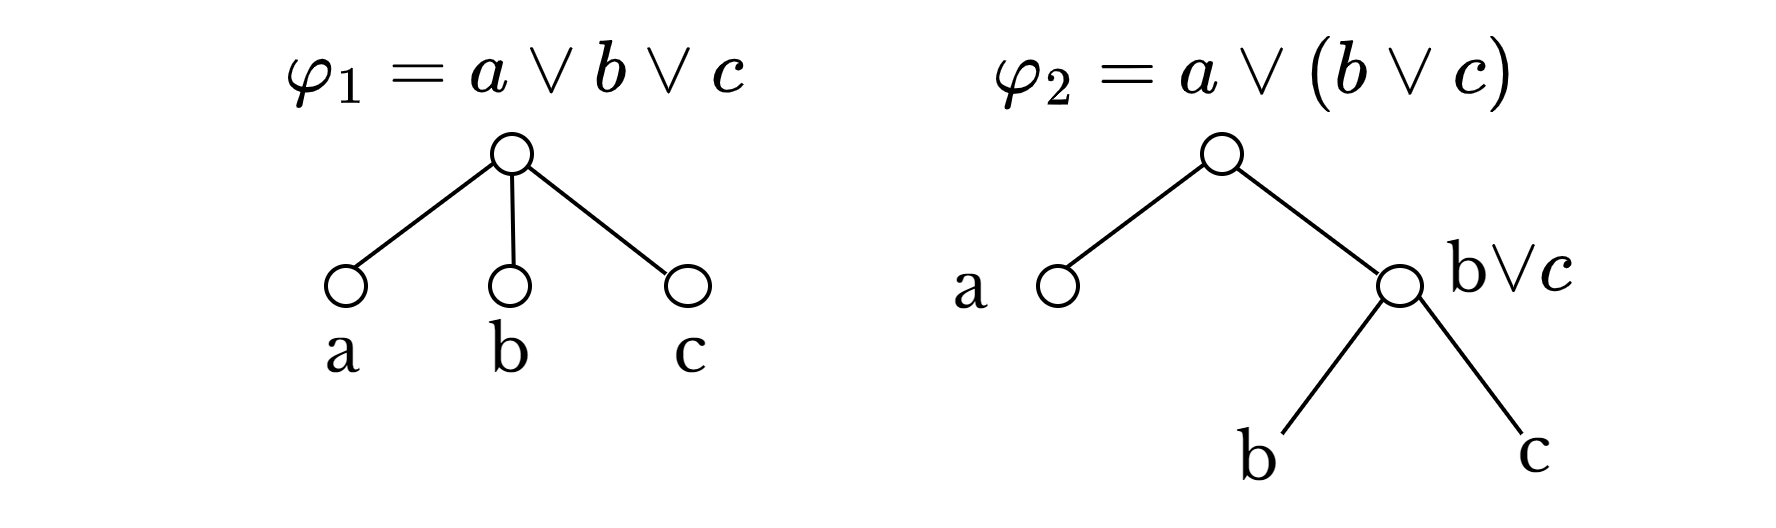
\includegraphics[scale=0.7]{flatten.png}
    \vspace{-0.4cm}
    \caption{STL trees for two logically equivalent formulas}
    \label{flatten}
    \vspace{-0.6cm}
\end{figure} 
\vspace{-0.2cm}

\subsection{Strategy encoding and feature vector}

Consider an STL specification $\varphi_1=\Box_{[1,T]}\lnot O\wedge \Diamond_{[1,T]}G$. Using the formula flattening method, the specification $\varphi_1$ can be compacted as $\hat{\varphi_1}$, which is shown as fig.\ref{always_eventually}. Now we take the STL tree decomposition step according to fig.\ref{stl_tree_decomposition}, and create SOS1 encoding for the $\vee$-type node in the STL tree (the red dotted line), 

The input feature vector $\theta^\varphi $ consists of the initial state $(x_0,v_0) \in \mathbb{R}^4$, coordinates of the obstacle and the goal area $X^o,X^g=(x^{min},x^{max},y^{min},y^{max}) \in \mathbb{R}^4$. Here we do not decompose the STL strategy and introduce the one-hot code since none of the repetitive structure appears. The SOS1 encoding $X^{SOS1}= [[X^{SOS1}]_1, [X^{SOS1}]_2]$ consists of two lists where $[X^{SOS1}]_1 \in \{0,1\}^{\log_2TN_f}$, $[X^{SOS1}]_2 \in \{0,1\}^{\log_2T}$. Thus, the input vector $\theta_{j}^{\varphi} = [x_0,v_0,X^o,X^g]$, and the label $\mathcal{S}_{j}(\theta^{\varphi})= [\mathcal{T}^{\pi}(\theta_{j}^{\varphi}), X_{j}^{SOS1}]$ where $j \in\{1,...,N\}$. $\mathcal{T}^{\pi}(\theta_{j}^{\varphi})\in \mathbb{R}$ is the index of tight constraints. Although this STL formula is not a complicated case, we still present the broad applicability and effectiveness of the proposed OMISTL method, which provides the potential to be combined with more complex STL formulas.

\begin{figure}[htbp] \centering 
    \vspace{0.5cm}
    \centering
    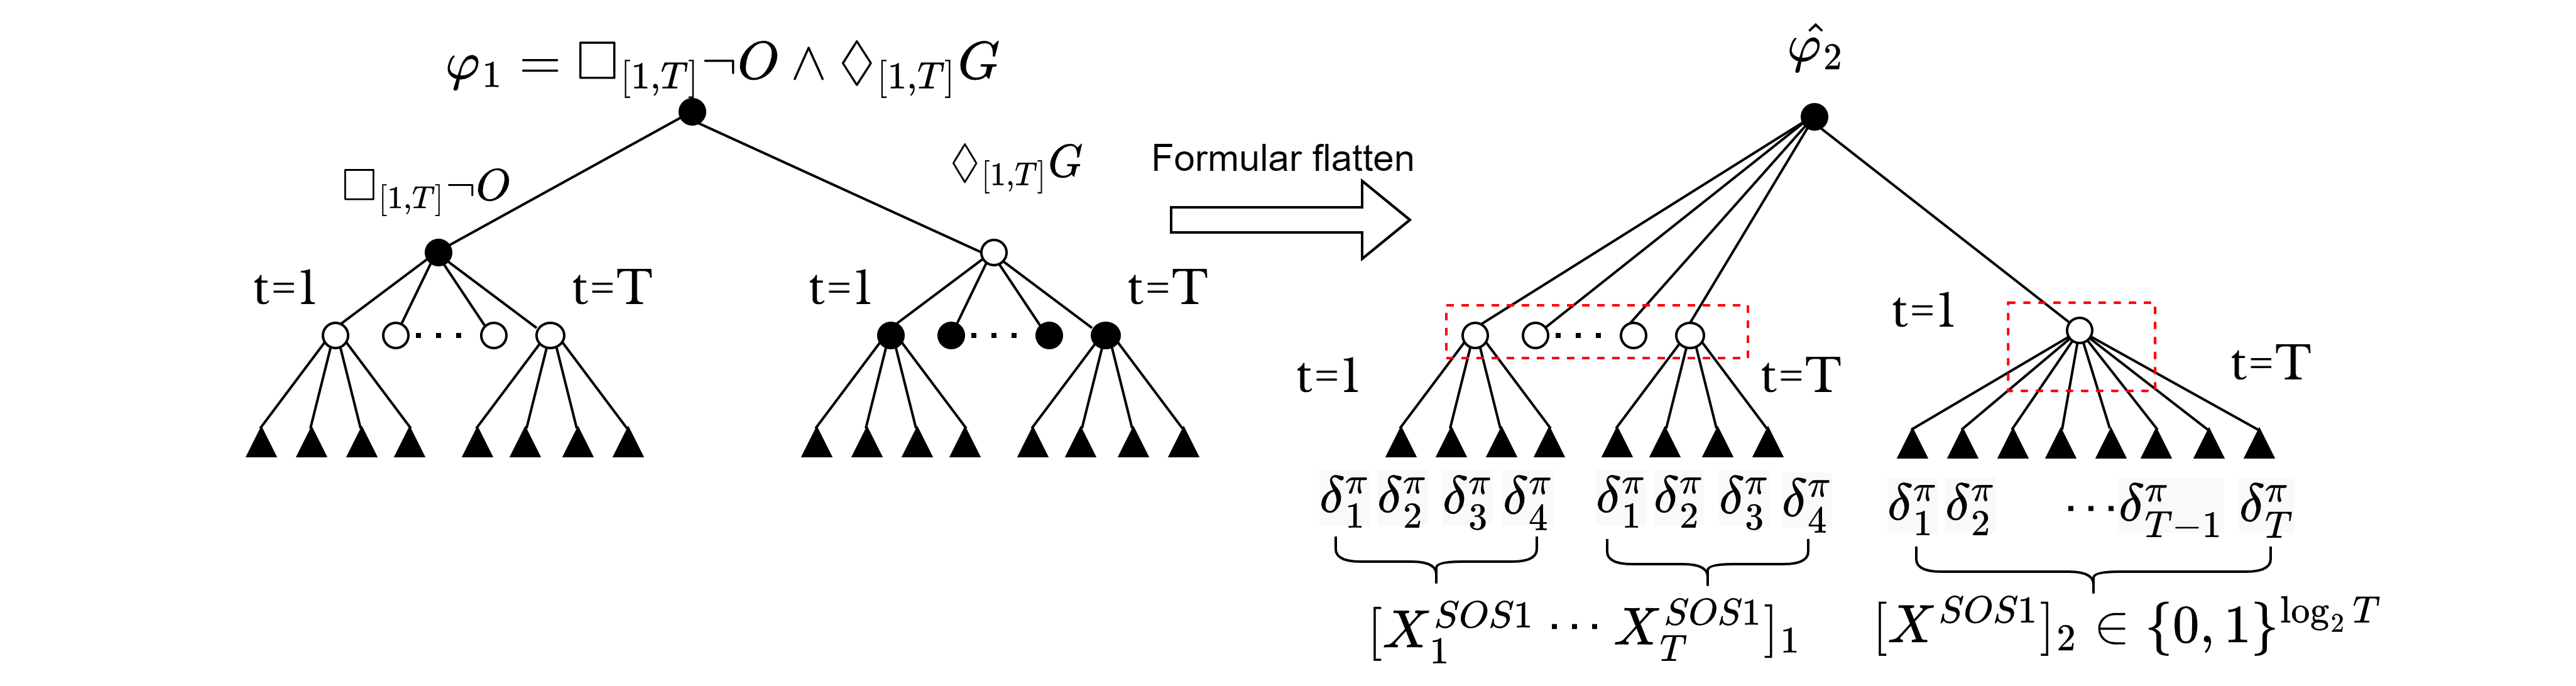
\includegraphics[scale=0.55]{alawasy_eventually.png}
    \vspace{-0.4cm}
    \caption{Formula flatten and SOS1 encoding for $\varphi_1=\Box_{[1,T]}\lnot O\wedge \Diamond_{[1,T]}G$ }
    \label{always_eventually}
    \vspace{-0.6cm}
\end{figure} 

\section{Supervised machine learning}
We deploy Feedforward Neural Network (FNN) to implement the classification task. FNN consists of $L$ layers and is defined as:
\begin{equation}
    \hat{s} = h_L(h_L-1(...h_1(\theta)))
\end{equation}
where each inner layers feature a ReLU function, $y_l=h_l(y_{l-1})=\sigma_l(W_ly_{l-1}+b_l), i=1,...,L$. The input $y_0=\theta$ and output $y_L = \hat{s}$, and for the output layer we use softmax function to provide a ranking between strategies.

For the loss function, the cross-entropy loss is used as :

\begin{equation}
    \mathcal{L}_{FNN}= \sum_{i=1}^{N}\sum_{j=1}^{m}(-s_{i,j})^T\log(\hat{s}_{i,j}) 
\end{equation}
where log is intended elementwise. This loss $\mathcal{L}$ can also be interpreted as the distance between the predicted probability density of the labels and to the true one. The training step consists of applying the classic stochastic
gradient descent with the derivatives of the cost function obtained using the back-propagation rule.


\chapter{Case studies}
\section{Parameter setting}

In this section, we numerically validate our OMISTL approach on the two proposed STL motion planning problems in robotics, one is the MPC control with obstacle avoiding specification, and the other considering robustness satisfaction is combined with STL specification $\varphi_1=\Box_{[1,T]}\lnot O\wedge \Diamond_{[1,T]}G $. The OMISTL which is implemented in Python and integrated with CVXPY to model the optimization problems is available at \cite[]{OMISTL_git}.

We adopt a double-integrator dynamics system in both the horizontal and vertical directions: 
$
\boldsymbol{x}=\left[p_{x}, p_{y}, v_{x}, v_{y}\right]^{T}, \boldsymbol{u}=\left[{u}_{x}, {u}_{y}\right]^{T}
$
where $p_{x}$ is the horizontal position of the robot and $p_{y}$ is the vertical position. The output signal is defined as $\boldsymbol{y}=\left[p_{x}, p_{y},v_x,v_y,u_x,u_y\right]^{T}$, giving us dynamics:
$$
A=\left[\begin{array}{ll}
I & I \\
0 & I
\end{array}\right], \quad B=\left[\begin{array}{l}
0 \\
I
\end{array}\right], \quad C=\left[\begin{array}{ll}
I & 0
\end{array}\right], \quad D=0 .
$$

State and input constraints $X$ and $U$ are defined to enforce maximum acceleration and velocity of $0.5 \mathrm{~m} / \mathrm{s}^{2}$ and $1 \mathrm{~m} / \mathrm{s}$ :
$$
\begin{aligned}
&X=\left\{\boldsymbol{x}\left|0 \leq p_{x} \leq 15,0 \leq p_{y} \leq 15,\right| p_{x}|\leq 1,| p_{y} \mid \leq 1\right\} . \\
&U=\left\{\boldsymbol{u}|| u_{x}|\leq 0.5,| u_{y} \mid \leq 0.5\right\}.
\end{aligned}
$$For each problem, we first solve a sufficient number of problems to generate the dataset. For each problem, we sample 20000 parameters $\theta^\varphi$ to collect the strategies and separate 90\% of the problems for training and the remaining 10\% for testing. We implemented a standard feedforward network with three layers, with each layer containing 128 neurons. The learning parameter settings are following in \cite{Cauligi2020}: the learning rate $r$=10e-4, batch size $B$=64, and number of epochs $E$=500. For comparison, we take the state-of-the-art STL encoding in \cite[]{kurtz2022mixed}, the previous learning-based frameworks CoCo\cite[]{Cauligi2020} \ and MLOPT \cite[]{bertsimas2022online} as the benchmarks, all of them implementing in python and CVXPY, and solving by Gurobi 9.1.2.

We run the experiments on the Intel(R) Core(TM) i7-8750H CPU @ 2.20GHz Laptop with 12 cores for the data collection involving the solution of the problem and an NVIDIA 1070max-q GPU for the neural network training. 

\section{Multiple obstacles avoiding examples}
\subsection{Model predictive control with obstacles avoidance}
For the MPC control problem, the prediction horizon $T$ is set to 10 and the number of obstacles $n$ to 5, while using typical encoding approach gives $n\cdot T\cdot N_f = 200$ integer variables \cite[]{2019Formal}, using our STL tree decomposition method yielding total $n\cdot T\cdot \log_2N_f = 100$ binary variables which is a half of that number, note that for general STL the number is $n\cdot T\cdot \log_2(N_f+1)$, because we have to introduce one more binary variable for each parent node. Here we can ignore the parent node because the STL tree only has two layers, and all of the parent nodes are combined with 'AND' relation, so we can list the constraints together and no need to introduce the parent node to represent the subformula holds or not.

The parameter space $\theta^\varphi \in \mathbb{R}^{37}$ for this problem included the initial and final states $x_0,x_g \in \mathbb{R}^4$ and coordinates $X_i^o \in \mathbb{R}^4$ of each obstacle, and a one-hot encoding of the obstacle index $X_i^{oh}$. Here the obstacle index is also taken as a part of the parameter because we decompose the STL strategies into different sub-strategies based on the different obstacles. As a last step, the network will predict a single sub-strategy for each obstacle, so the index should be sampled to recover the original strategy, the detailed explanation can be found in \ref{Strategy encoding and feature vector}.

 We set three reference points for the MPC problem, and make the robot travel recurrently following these points. When the robot reaches a new reference point, it changes the target to the next reference point. The sampling time is set to 0.1 sec, which means the OMISTL must provide solutions within 0.1 sec to operate the system properly. The prediction horizon is T = 10, and the horizon length of the total trajectory is set as 610, which means the problem will be solved 600 times in total. 
 The trajectory is shown in Fig.\ref*{mpc_route}, it takes 3.641s to solve the recursive problems, and at each timestep, we spend only 0.0061s to return the solution on average. Though there seem existing some constraint violations due to the marginal between sampling time, our proposed OMISTL allows its real-time implementation on the robot control in practice.

 \begin{figure}
    % \vspace{0.5cm}
    \centering
    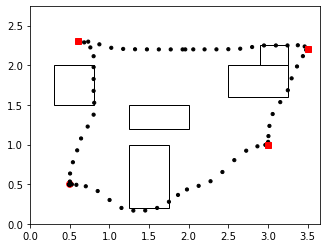
\includegraphics[scale=0.6]{mpc_route.png}
    \vspace{-0.4cm}
    \caption{
    Trajectory planning example with 5 obstacles and sampling time 0.1sec, the red points represent the reference points of MPC}
    \label{mpc_route}
    \end{figure}

 \subsection{Results evaluation}
Let us examine the performance of solving MICP online with the proposed OMISTL. The problem setting refers to the trajectory planning example in \cite[]{bertsimas2022online}, where the different numbers of obstacles and prediction horizon lengths are applied here. The performance of the learning-based framework can be evaluated from two indicates: the feasibility, defined as the percentage of feasible solutions in the test dataset; the optimality, defined as the ratios of the obtained and the optimal costs (returned by Gurobi). The results are plotted in fig.\ref*{Performance of OMISTL}. 

Firstly, figures (a) and (b) respectively show the solve time performed with the learning-based OMISTL and the state-of-the-art solver Gurobi. The results demonstrate that OMISTL consistently outperforms Gurobi in all problem settings, where the solving time is always within 0.1s. Not surprisingly, the increasing number of obstacles and horizons results in more computation time for both approaches, which conforms with intuitions. The remarkable thing is that, while increasing the problem sizes, the growth trend of OMISTL solving time is not as sensitive as Gurobi. Because the OMISTL computation complexity is only involved with evaluating the network and solving a CO problem, and Gurobi has to deal with a MICP that may have exponentially growing complexity. Moreover, it is very important to remark the reliability of the computation time required by our approach. The execution time of Gurobi with branch-and-bound algorithms greatly depends on how the solution tree is searched and pruned. This can vary significantly when problem parameters change, making the whole online computation unreliable in real-time applications. Whereas, the results indicate our approach always returns a feasible solution within 0.1s reliably in terms of all problem parameters.

Secondly, figure \ref{Performance of OMISTL} (c) demonstrates how the feasibility changes with the increasing size of the problem. The best feasibility is naturally obtained when there are 5 obstacles, and the horizon is 6, with 92.83\% feasible solutions. As expected, the number of feasible solutions decreases continuously with the increasing obstacles and time horizons. An accidental increase might be attributed to a good problem setting or a well-trained network. The number of integer strategies has witnessed a significant increase with the growth of problem sizes as in \ref{Performance of OMISTL} (d). This observation is also compatible with the explanation for why we prefer fewer binary variables, i.e., the more binary variables we introduce, the more the resulting strategies and the label types, and the worse the network performance. 

\begin{figure*}[!htb]
        \centering
        \subfigure[OMISTL solve time]{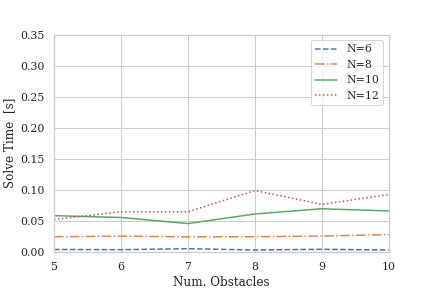
\includegraphics[width=0.45\hsize, height=0.35\hsize]{solve_time_ML.png}}
        \subfigure[Gurobi solve time]{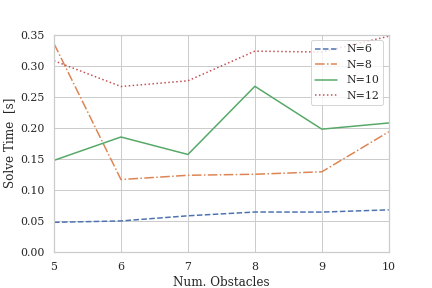
\includegraphics[width=0.45\hsize, height=0.35\hsize]{solve_time_gurobi.png}}
    
        \subfigure[Percentage of feasible solutions]
        {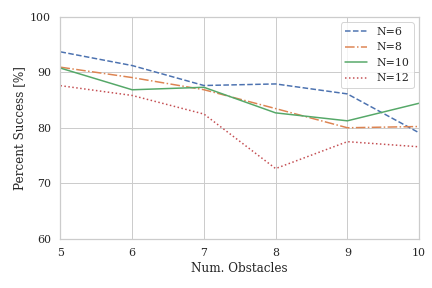
\includegraphics[width=0.45\hsize, height=0.35\hsize]{percent_success_mpc.png}}
        \subfigure[Number of strategies]{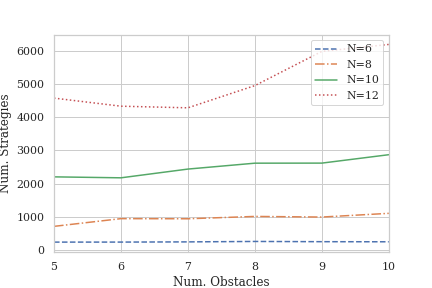
\includegraphics[width=0.45\hsize, height=0.35\hsize]{num_strategies.png}}
        \caption{Evaluation of OMISTL and MLOPT with different horizons}
    \label{Performance of OMISTL}
    \end{figure*}

Lastly, the optimality of solutions is present in the bar chart \ref{cost_ratios}, where the length of bars represents the solution quality. The higher bars imply the worse solutions since they are farther from the optimal solutions, where the bar length equals 100, meaning that the predicted solution is as good as the optimal solutions. Although the increasing horizons may cause a slight loss of the solution optimality, no evident correlation can be found between the solution optimality and the obstacles numbers, which illustrates the excellent scalability of the proposed learning-based framework. OMISTL finds almost all the optimal solutions within 0.1s, where the suboptimal cost is not exceeding 105\% of the optimal cost.

 \begin{figure}
    % \vspace{0.5cm}
    \centering
    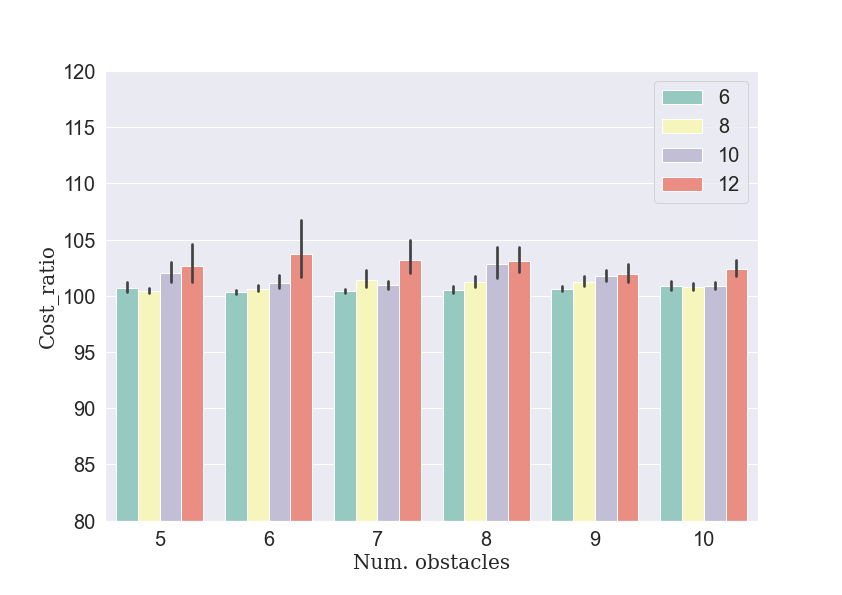
\includegraphics[scale=0.25]{cost_ratios.png}
    \vspace{-0.4cm}
    \caption{Solution optimality analysis}
    \label{cost_ratios}
    \end{figure}

\subsection{ Encoding comparison}

The good results of our framework are naturally obtained first thanks to the great ability of machine learning to predict the integer solutions. More importantly, our proposed efficient STL encoding based on the STL tree plays a significant role in the reduction of binary variables and integer strategies. This efficient encoding is beneficial to not only the offline computation when sampling problems, but also the online prediction because it improves the accuracy by reducing the strategies. 

To illustrate the encoding performance, we set the multiple obstacles avoiding examples and compare OMISTL with the learning-based method MLOPT \cite[]{bertsimas2022online}, which uses the typical encoding without STL consideration. We use the default problem parameters with five obstacles and apply the different time horizons on both methods. The results are concluded in \ref{encoding_comparision}. 

The first thing we notice is that the integer variables of OMISTL are merely half of the MLOPT, while the number of total variables and constraints is more than MLOPT. Because our proposed encoding introduces more continuous variables and constraints to define the SOS1 constraints. Secondly, since the MICP computation bottlenecks are largely depending on the integer variables, the increase of continuous variables and constraints imposes a trivial penalty on the computation. However, it brings us fewer binary variables and strategies, contributing to the offline part and online part, which is a good deal.

\begin{table}[]
    \begin{center}
    \scalebox{0.80}{
    \begin{tabular}{cccccccc}
    \hline
    N                                  &        & 5    & 10   & 15    & 20    & 25    & 30    \\ \hline
    \multirow{2}{*}{Integer variables} & OMISTL & 50   & 100  & 150   & 200   & 250   & 300   \\
                                       & MLOPT  & 100  & 200  & 300   & 400   & 500   & 600   \\ \hline
    \multirow{2}{*}{Total variables}   & OMISTL & 184  & 364  & 544   & 724   & 904   & 1084  \\
                                       & MLOPT  & 134  & 264  & 394   & 524   & 654   & 784   \\ \hline
    \multirow{2}{*}{Constraints}       & OMISTL & 384  & 759  & 1134  & 1509  & 1884  & 2259  \\
                                       & MLOPT  & 184  & 359  & 534   & 709   & 884   & 1059  \\ \hline
    \multirow{2}{*}{Strategy number}   
                                       & OMISTL  & 241  & 940  & 4436  & 9758  & 12291 & 19021 \\
                                       & MLOPT & 3536 & 8329 & 13990 & 17892 & 24421 & 29542 \\ \hline
    \end{tabular}}          
    \end{center}
\caption[]{Encoding comparison in different horizons}
\label{encoding_comparision}
\end{table}

\subsection{Learning-based methods comparison}

Using the setting of motion planning problem in the learning-based framework CoCo \cite[]{Cauligi2020}, we compute the problem 1000 times and take the average value. The conclusions are as follows.

Firstly, Fig.\ref{comparision} shows that our proposed OMISTL can report more than 90\% feasible solutions, which is more than the other two learning-based approaches, CoCo for 85.27\% and MLOPT for 34.35\%, and is merely less than Gurobi with 98\%. Because Gurobi always returns a feasible solution at optimality. However, our approach spends less time solving the MICP, with more than 91.67\% of solutions being globally optimal. Secondly, although the solving time is sometimes slightly more than CoCo and MLOPT due to the SOS1 constraints we used in efficient STL encoding, OMISTL returns more optimal solutions than CoCo and MLOPT as compensation. All the three learning-based approaches obtain a considerable reduction on the solving time compared with Gurobi, and MLOPT wins the best solving time by a narrow margin. Fortunately, it implies that the computation is not 
obviously affected by the introduction of SOS1 constraints in OMISTL. In addition, MLOPT reports approximately 67,000 strategies compared to 129 for OMISTL and 224 for CoCo, gaining the worst performance with 34.35\% feasible solutions. This huge gap is attributable to the fact that MLOPT does not decompose the strategies, while OMISTL and CoCo apply their corresponding ways to simplify the integer strategies. Finally, the outperformance of OMISTL compared with CoCo results from the efficient STL encoding, which further reduces the number of integer strategies, allowing for better supervision of the classifier since more data are available per class.

\begin{figure*}[!htb]
    \centering
    \subfigure[Percentage of success]{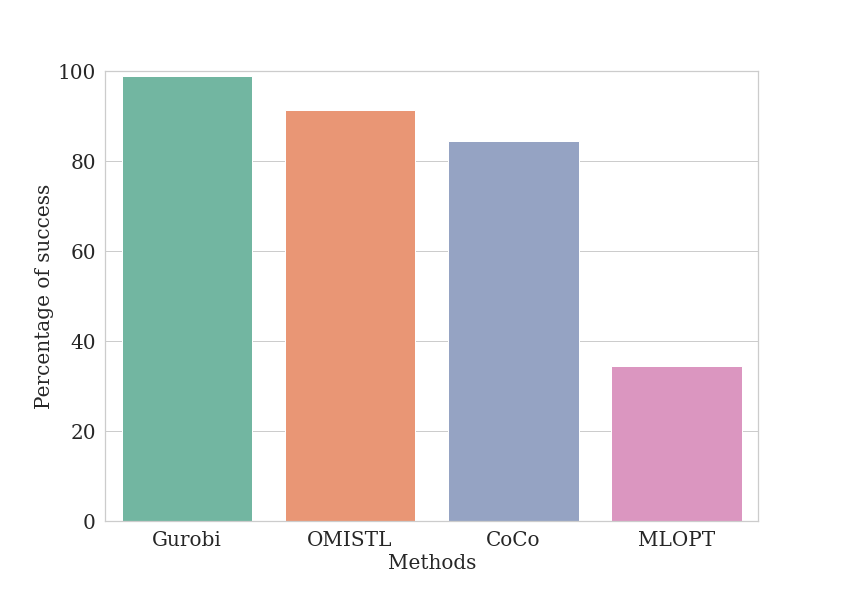
\includegraphics[width=0.45\hsize, height=0.3\hsize]{percent_compare_ratios.png}\label{percent_compare_ratios}}\hspace{0.1cm}
    \subfigure[Solve time]{\includegraphics[width=0.45\hsize, height=0.3\hsize]{Solve_time_compare.png}\label{solve_time}}
    \subfigure[Relative cost]{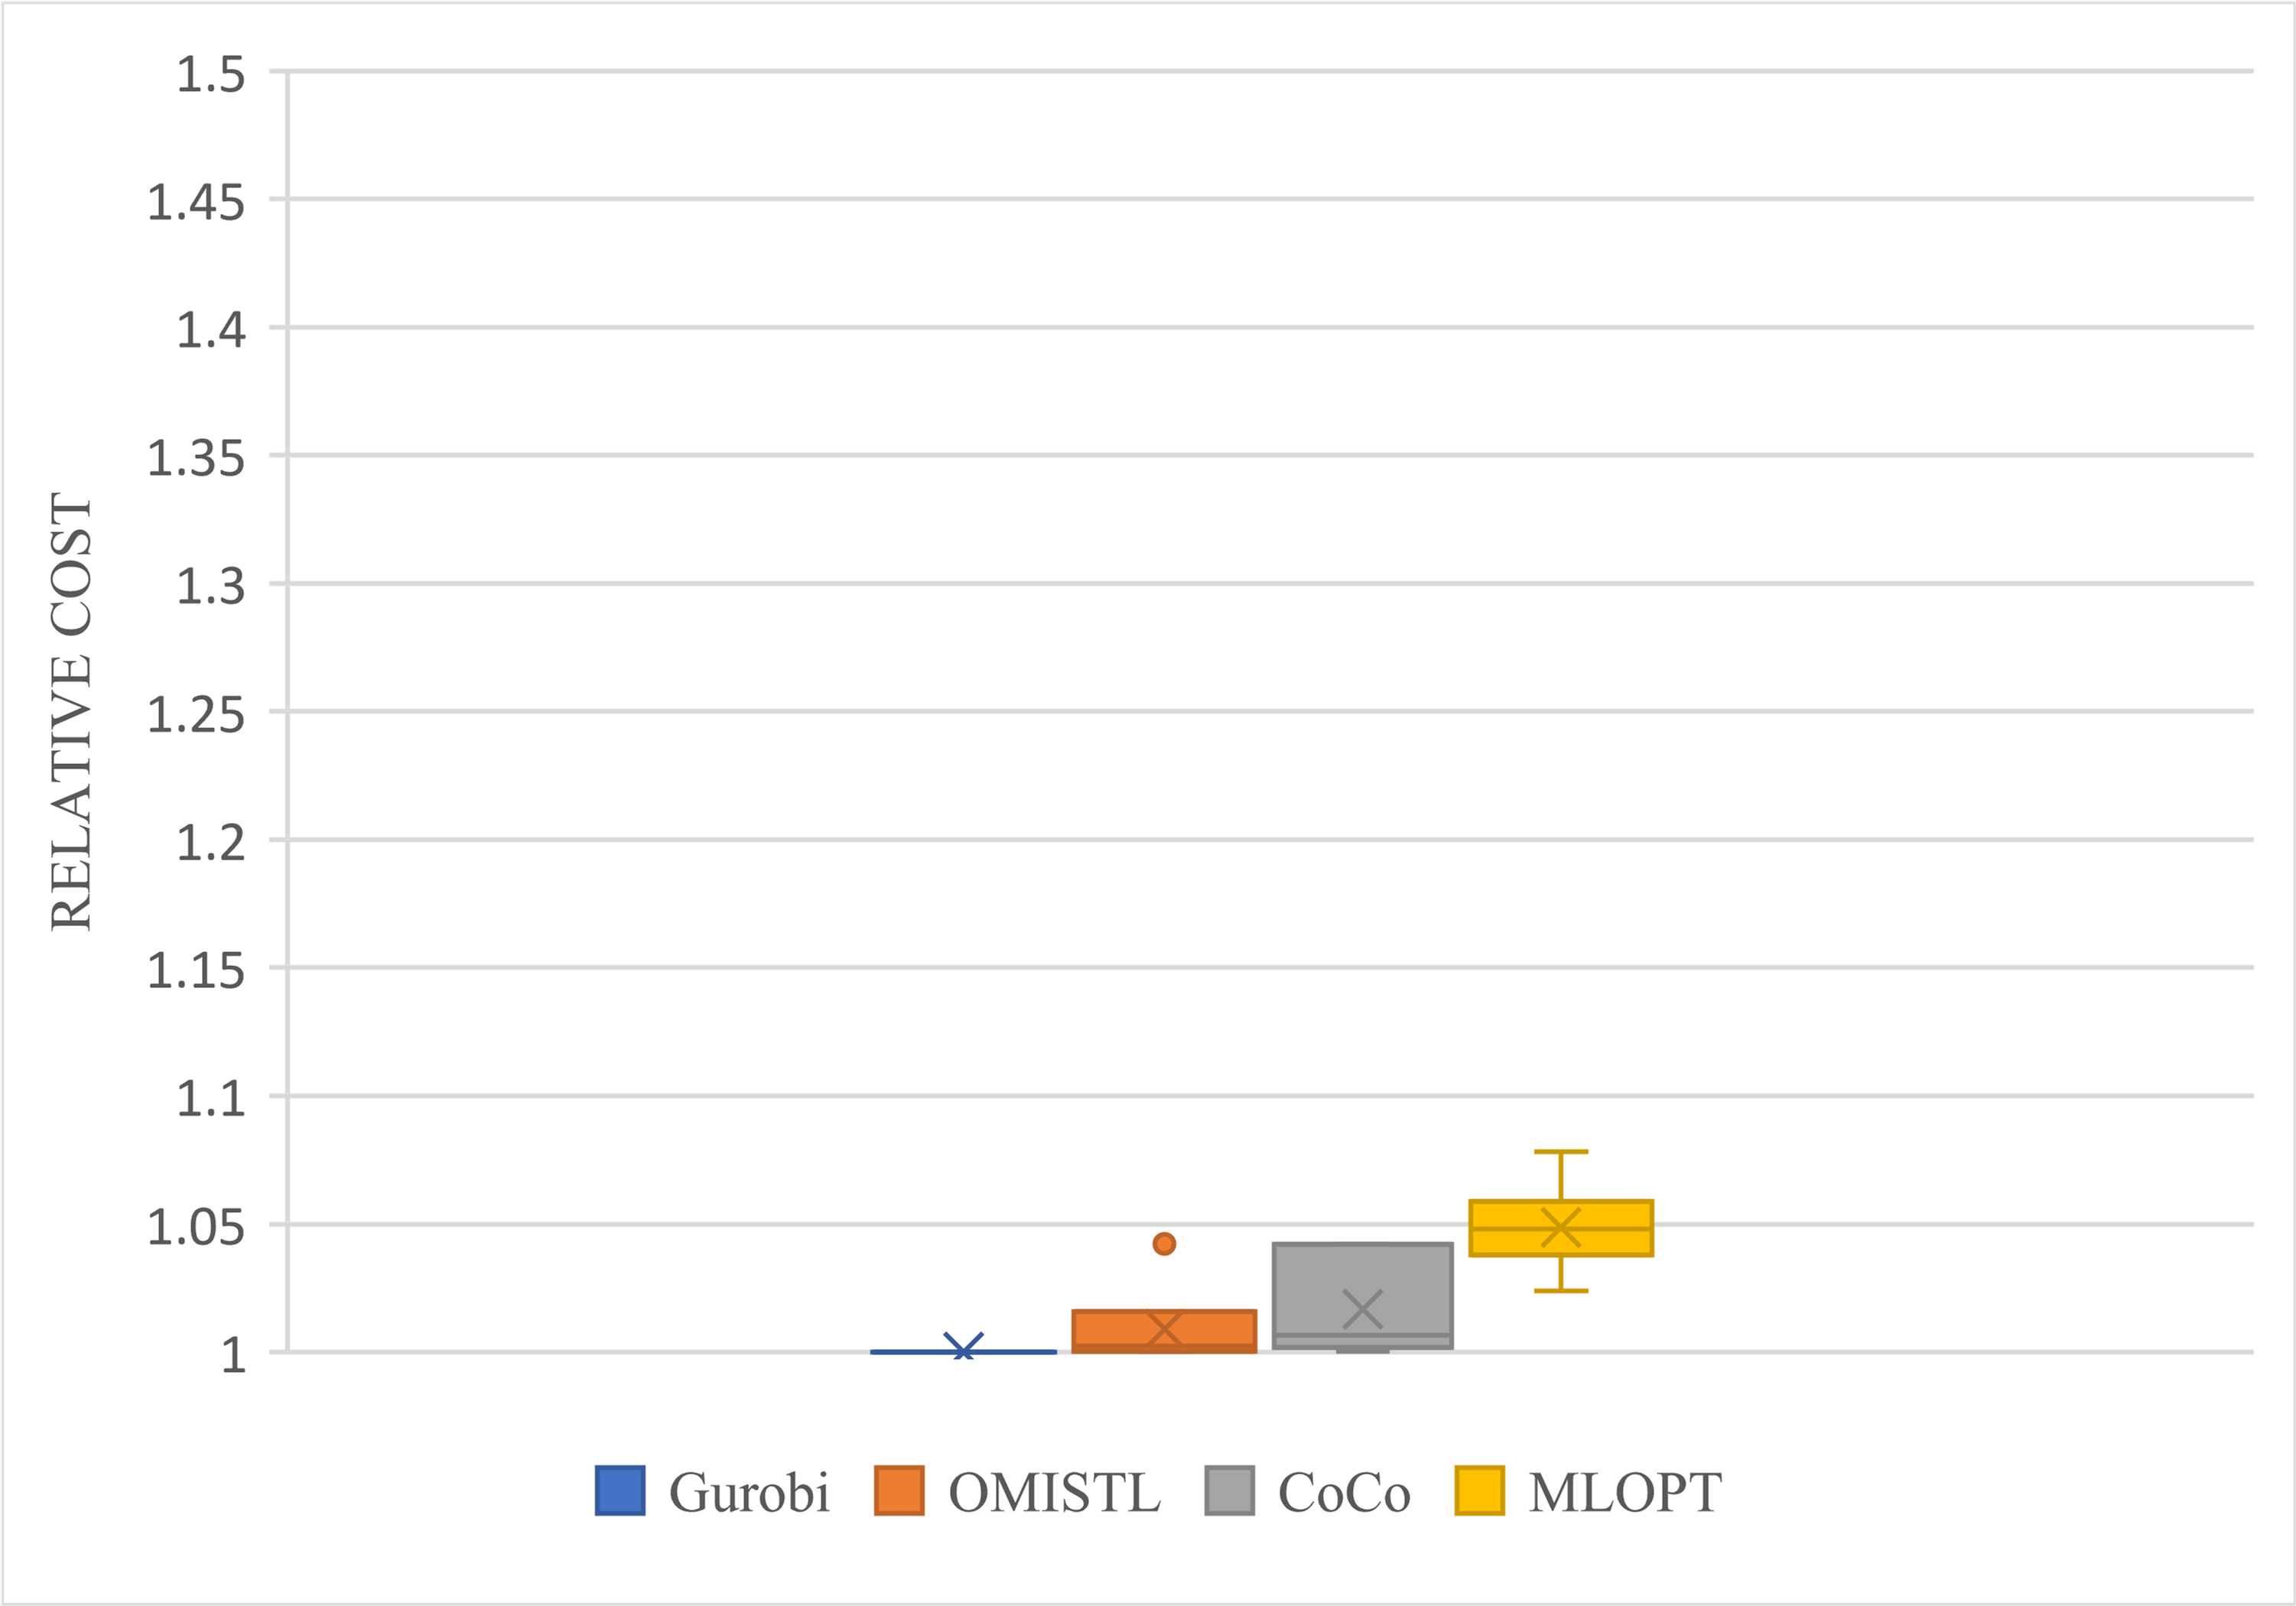
\includegraphics[width=0.45\hsize, height=0.3\hsize]{Relative_cost.png}\label{Relative_cost}}
    \subfigure[Number of strategies]{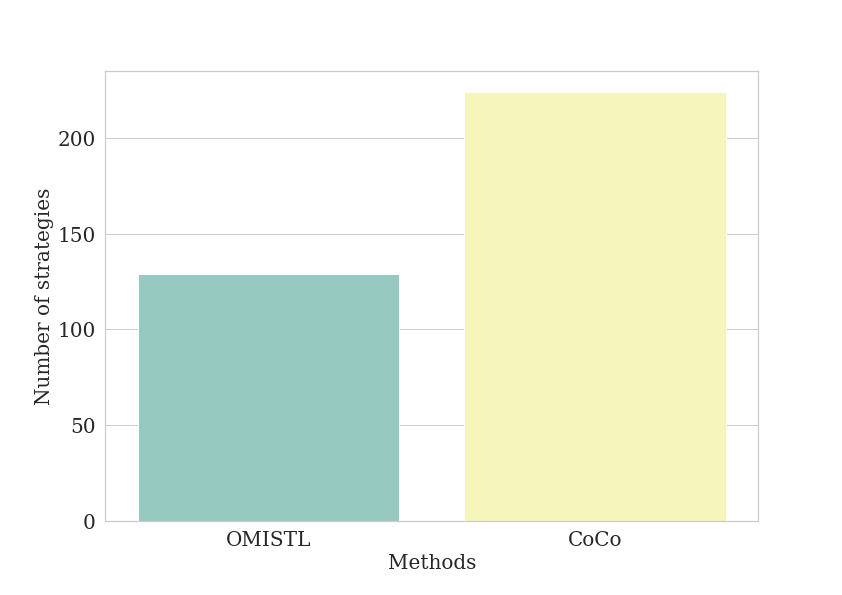
\includegraphics[width=0.45\hsize, height=0.3\hsize]{number_strategy_methods.png}\label{number_strategy_methods}}
    \caption{Comparison with Gurobi and learning-based approaches}
    \label{comparision}
\end{figure*}


\section{Results of the example of STL planner with robustness}

\subsection{ STL setting}
We finally provide three examples to demonstrate a  widespread application of  OMISTL on STL formulas.  Thanks to the efficient STL encoding and STL integer strategy, one can extend the learning-based framework into more general STL scenarios.

The first obstacle avoidance example, written as $\varphi_1=\Box_{[0,10]}(\bigwedge_{i=1}^5\lnot O_i)$, comes from the MPC problem, and the only difference is that we do not solve it recursively. Referring to \cite{kurtz2022mixed}, we set another two benchmarks to show the great potential of OMISTL on general STL formulas. The first STL specification is written as:
\begin{equation}
    \varphi_2=\Box_{[1,10]}\lnot O\wedge \Diamond_{[1,10]}G 
\end{equation}
in this scenario, the mobile robot must avoid an obstacle, and gradually reach the target area which is plotted as green for at least 10 timesteps, as shown in Fig.\ref{alway_eventually_route}. Recall that this STL motion planning problem cannot be solved with the typical motion planning MICP encoding, since it is related to temporal relations. 

\begin{figure}
    % \vspace{0.5cm}
    \centering
    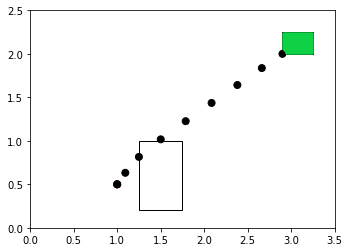
\includegraphics[scale=0.6]{always_eventually_route.png}
    \caption{Alway eventually example with specification $\varphi_2=\Box_{[1,10]}\lnot O\wedge \Diamond_{[1,10]}G $}
    \label{alway_eventually_route}
\end{figure}

We design a more complex multi-target motion task in the second STL specification, as shown in Fig.\ref{multi_targets}. In this setting, there are three groups of targets $T^j (j=1,2,3)$, where each group contains two targets that are plotted with the same color. And The robot must eventually reach one of two possible goals in addition to avoiding obstacles, which can be written as:
\begin{equation}
    \varphi_3=\bigwedge_{i=1}^3\left(\bigvee_{j=1}^2 \Diamond_{[0, T]} T_i^j\right) \wedge \square_{[0, T]}(\neg O)
\end{equation}
where $T_i^j$ represents the $j_{th}$ target in $i_{th}$ group.

\begin{figure*}[!htb]
    \centering
    \subfigure[]{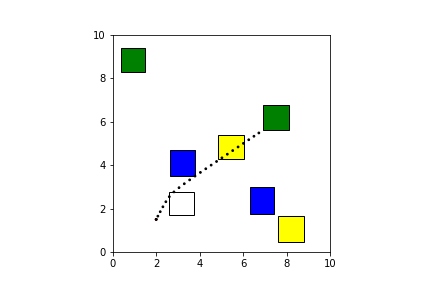
\includegraphics[scale=0.3]{multi_targets1.png}}
    \subfigure[]{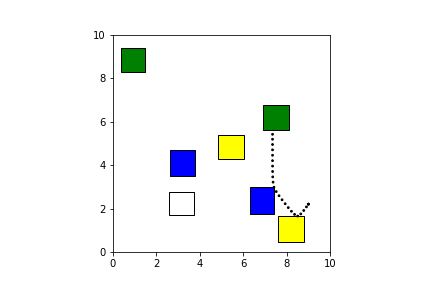
\includegraphics[scale=0.3]{multi_targets2.png}}
    \subfigure[]{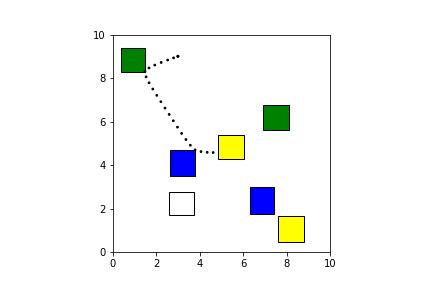
\includegraphics[scale=0.3]{multi_targets3.png}}
    \subfigure[]{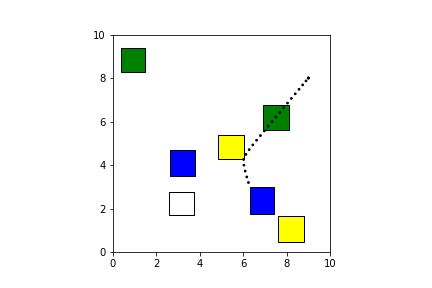
\includegraphics[scale=0.3]{multi_targets4.png}}
    \caption{Results of multi-target example }
    \label{multi_targets}
\end{figure*}

\subsection{Performance evaluation}

Different horizons are set to evaluate the performance of OMISTL on general STL formulas, and each problem is computed 1000 times and takes the average. The parameters and results of three STL specifications are shown in table \ref{benchmark_comparison}. 

Our first conclusion from this table \ref*{benchmark_comparison} are the following. For all of these specifications, our proposed approach uses fewer binary variables than the typical STL encoding \cite[]{2019Formal}\cite[]{Cauligi2020}. For obstacle avoidance example OMISTL only uses half of the binary variables in typical encoding (since four-face obstacles are considered, $N_f=4$ and $\log_2N_f=2 )$. Only a logarithmic number of binary variables are introduced in the other two benchmarks. 

Secondly, the more disjunctions in a disjunctive formula, the more binary variables are reduced using our STL encoding relative to the typical encoding, which can be understood by simple mathematics. Recall that we use a $\sum_{1}^{N^\lor}(\log_2(N_i+1))$ number of binaries, where $N_i$ is the number of disjunctions in a disjunctive formula. When we take the logarithm number of $N_i$, clearly increasing $N_i$ leads to fewer binaries compared with $T \cdot N_i$. This property not only makes OMISTL good scalability for large-size STL formulas, but also reveals a valuable insight, that is, we prefer increasing the number of disjunctions when designing the STL tasks. For instance, increasing the obstacle faces or horizons in $\diamond, \vee$ syntax. Especially in the multi-target example, a more significant reduction of binaries can be observed compared with the other two, because multi-target specification contains more disjunctions. 

Naturally, it arrives at the last conclusion that OMISTL gains speed-ups of 1-2 orders of magnitude when solving MICP online, and the acceleration effect largely depends on the number of binary variables and disjunctions. Surprisingly, OMISTL almost realizes a 400$\times$  speed up in the multi-target examples compared with the state-of-art solver Gurobi. As we have explained before, the multi-target STL formula contains many disjunctions, which causes difficulties when Gurobi tries to use branch-and-bound to explore the branches of the solution tree. However, OMISTL directly predicts the candidate integer solutions, avoiding exploring the complex tree structure. This is why OMISTL wins a significant advantage in the third specification.

It is also remarkable that there exists a trade-off between the number of disjunctions and the speed-up performance. While increasing the disjunctions of STL formulas can improve the relative performance of OMISTL, what follows is the increase of integer variables, which affects the network accuracy.


\begin{table}[!htbp]
    \scalebox{0.75}{
    \centering
    \begin{tabular}{c|c|c|cc|cc}
    Specifications                         & Horizon(T) & Disjunctions & \multicolumn{2}{c|}{Binary variables} & \multicolumn{2}{c}{Average Solve time(s)} \\
                                           &            & (maximum)           & Typical             & OMISTL             & Gurobi            & OMISTL            \\ \hline
    \multirow{3}{*}{Obstacle avoiding} & 10         & 4         & 200              & 100                & 0.1433             & 0.0214            \\
                                           & 15         & 4         & 300              & 150                & 0.2132             & 0.0226            \\
                                           & 20         & 4         & 400              & 200                & 0.2921             & 0.0245            \\ \hline
    \multirow{3}{*}{Always eventually}     & 10         & 10         & 50               & 34                 & 0.0463             & 0.0156            \\
                                           & 15         & 15         & 75              & 49                 & 0.0728             & 0.0158            \\
                                           & 20         & 20         & 100              & 65                & 0.1093             & 0.0162            \\ \hline
    \multirow{3}{*}{Multi-target}            & 15         & 30         &150              & 60                 & 1.0312             & 0.0336            \\
                                           & 20         & 40         & 200              & 78                 & 4.9011             & 0.0334            \\
                                           & 25         & 50         & 250             & 93               & 11.0621             & 0.0345           
    \end{tabular}}
    \caption[]{Comparison for three specifications}\label{benchmark_comparison}
    \end{table}
    Let us now give more details about the tight constraints. Another definition of the tight constraints in CoCo is used for comparison. Since CoCo cannot deal with STL formulas, the obstacle avoidance example is implemented where the problem parameters are referring to \cite[]{Cauligi2020}. The number of tight constraints varies from problem to problem, so we compute the average value over 1000 samplings and take the integer. The results are concluded in Table \ref*{tight_constraints}.

    Although OMISTL uses more constraints compared with CoCo, fewer tight constraints are obtained through our definition. Recall the property of SOS1 constraints, there is only one non-zero element in the SOS1 vector, and the constraint corresponding to that one element is defined as the tight constraint. Although the SOS1 constraints introduce additional continuous variables and constraints, our tight definition brings fewer tight constraints compared with CoCo, which matters a lot for network training. Moreover, the previous results demonstrate that adding a few continuous variables and constraints has little impact on the online computation, because solving a CO is already very fast. 
    

% Please add the following required packages to your document preamble:
% \usepackage{multirow}
\begin{table}[]
    \begin{center}
    
        \scalebox{0.80}{
            \begin{tabular}{c|c|cccccc}
                Number of obstacles     & Parameters        & 5   & 6   & 7   & 8   & 9   & 10  \\ \hline
                \multirow{3}{*}{OMISTL} & Total constaints  & 384 & 449 & 514 & 579 & 644 & 709 \\
                                        & Tight constraints & 30  & 36  & 42  & 48  & 54  & 60  \\
                                        & Strategy number   & 231 & 232 & 238 & 251 & 244 & 241 \\ \hline
                \multirow{3}{*}{CoCo}   & Total constaints  & 184 & 209 & 234 & 259 & 284 & 309 \\
                                        & Tight constraints & 66  & 81  & 94  & 107 & 121 & 134 \\
                                        & Strategy number   & 562 & 535 & 563 & 558 & 576 & 556 \\ \hline
                \end{tabular}
        }
        \caption[]{Comparison of constraints}
        \label{tight_constraints}
    \end{center}
    \end{table}

\chapter{Conclusion}

This work proposes a learning-based framework to solve the MPC and STL motion planning problems. The proposed efficient STL encoding approach leads to a number of binary variables that is logarithmic in the number of specification predicates, which significantly reduces the number of binary variables compared with the standard STL encoding. 

The numerical experiments demonstrate that the proposed OMISTL framework gains speed-ups of 1-2 orders of magnitude in online computation time, where the acceleration mainly depends on the integer variables and disjunctions of STL formulas. In almost all cases OMISTL always returns the solutions within 0.1s. In addition, the solution feasibility is better than the existing learning-based method with more than 90\% feasible solutions, where CoCo is 85.27\% and MLOPT is 34.35\%. And 92\% of them are globally optimal, comparing to Gurobi with 98\%. The proposed framework is, therefore, suitable for computing STL motion planning problems in real-time with high reliability and speed.

It is difficult to estimate the amount of samplings required to accurately learn the classification problem, which stll remains empirically. Future contributions will focus on providing theoretical guarantees on how to characterize the strategy space by effectively sampling the parameter space of the problems and
to bound the optimality gap of feasible solutions found online.

\bibliography{literature}


\sloppy  % force the page margins to be respected


\end{document}
